% Options for packages loaded elsewhere
\PassOptionsToPackage{unicode}{hyperref}
\PassOptionsToPackage{hyphens}{url}
\PassOptionsToPackage{dvipsnames,svgnames,x11names}{xcolor}
%
\documentclass[
  letterpaper,
  DIV=11,
  numbers=noendperiod]{scrreprt}

\usepackage{amsmath,amssymb}
\usepackage{iftex}
\ifPDFTeX
  \usepackage[T1]{fontenc}
  \usepackage[utf8]{inputenc}
  \usepackage{textcomp} % provide euro and other symbols
\else % if luatex or xetex
  \usepackage{unicode-math}
  \defaultfontfeatures{Scale=MatchLowercase}
  \defaultfontfeatures[\rmfamily]{Ligatures=TeX,Scale=1}
\fi
\usepackage{lmodern}
\ifPDFTeX\else  
    % xetex/luatex font selection
\fi
% Use upquote if available, for straight quotes in verbatim environments
\IfFileExists{upquote.sty}{\usepackage{upquote}}{}
\IfFileExists{microtype.sty}{% use microtype if available
  \usepackage[]{microtype}
  \UseMicrotypeSet[protrusion]{basicmath} % disable protrusion for tt fonts
}{}
\makeatletter
\@ifundefined{KOMAClassName}{% if non-KOMA class
  \IfFileExists{parskip.sty}{%
    \usepackage{parskip}
  }{% else
    \setlength{\parindent}{0pt}
    \setlength{\parskip}{6pt plus 2pt minus 1pt}}
}{% if KOMA class
  \KOMAoptions{parskip=half}}
\makeatother
\usepackage{xcolor}
\ifLuaTeX
  \usepackage{luacolor}
  \usepackage[soul]{lua-ul}
\else
  \usepackage{soul}
  
\fi
\setlength{\emergencystretch}{3em} % prevent overfull lines
\setcounter{secnumdepth}{5}
% Make \paragraph and \subparagraph free-standing
\ifx\paragraph\undefined\else
  \let\oldparagraph\paragraph
  \renewcommand{\paragraph}[1]{\oldparagraph{#1}\mbox{}}
\fi
\ifx\subparagraph\undefined\else
  \let\oldsubparagraph\subparagraph
  \renewcommand{\subparagraph}[1]{\oldsubparagraph{#1}\mbox{}}
\fi


\providecommand{\tightlist}{%
  \setlength{\itemsep}{0pt}\setlength{\parskip}{0pt}}\usepackage{longtable,booktabs,array}
\usepackage{calc} % for calculating minipage widths
% Correct order of tables after \paragraph or \subparagraph
\usepackage{etoolbox}
\makeatletter
\patchcmd\longtable{\par}{\if@noskipsec\mbox{}\fi\par}{}{}
\makeatother
% Allow footnotes in longtable head/foot
\IfFileExists{footnotehyper.sty}{\usepackage{footnotehyper}}{\usepackage{footnote}}
\makesavenoteenv{longtable}
\usepackage{graphicx}
\makeatletter
\def\maxwidth{\ifdim\Gin@nat@width>\linewidth\linewidth\else\Gin@nat@width\fi}
\def\maxheight{\ifdim\Gin@nat@height>\textheight\textheight\else\Gin@nat@height\fi}
\makeatother
% Scale images if necessary, so that they will not overflow the page
% margins by default, and it is still possible to overwrite the defaults
% using explicit options in \includegraphics[width, height, ...]{}
\setkeys{Gin}{width=\maxwidth,height=\maxheight,keepaspectratio}
% Set default figure placement to htbp
\makeatletter
\def\fps@figure{htbp}
\makeatother

\KOMAoption{captions}{tableheading}
\makeatletter
\@ifpackageloaded{tcolorbox}{}{\usepackage[skins,breakable]{tcolorbox}}
\@ifpackageloaded{fontawesome5}{}{\usepackage{fontawesome5}}
\definecolor{quarto-callout-color}{HTML}{909090}
\definecolor{quarto-callout-note-color}{HTML}{0758E5}
\definecolor{quarto-callout-important-color}{HTML}{CC1914}
\definecolor{quarto-callout-warning-color}{HTML}{EB9113}
\definecolor{quarto-callout-tip-color}{HTML}{00A047}
\definecolor{quarto-callout-caution-color}{HTML}{FC5300}
\definecolor{quarto-callout-color-frame}{HTML}{acacac}
\definecolor{quarto-callout-note-color-frame}{HTML}{4582ec}
\definecolor{quarto-callout-important-color-frame}{HTML}{d9534f}
\definecolor{quarto-callout-warning-color-frame}{HTML}{f0ad4e}
\definecolor{quarto-callout-tip-color-frame}{HTML}{02b875}
\definecolor{quarto-callout-caution-color-frame}{HTML}{fd7e14}
\makeatother
\makeatletter
\@ifpackageloaded{bookmark}{}{\usepackage{bookmark}}
\makeatother
\makeatletter
\@ifpackageloaded{caption}{}{\usepackage{caption}}
\AtBeginDocument{%
\ifdefined\contentsname
  \renewcommand*\contentsname{Table of contents}
\else
  \newcommand\contentsname{Table of contents}
\fi
\ifdefined\listfigurename
  \renewcommand*\listfigurename{List of Figures}
\else
  \newcommand\listfigurename{List of Figures}
\fi
\ifdefined\listtablename
  \renewcommand*\listtablename{List of Tables}
\else
  \newcommand\listtablename{List of Tables}
\fi
\ifdefined\figurename
  \renewcommand*\figurename{Figure}
\else
  \newcommand\figurename{Figure}
\fi
\ifdefined\tablename
  \renewcommand*\tablename{Table}
\else
  \newcommand\tablename{Table}
\fi
}
\@ifpackageloaded{float}{}{\usepackage{float}}
\floatstyle{ruled}
\@ifundefined{c@chapter}{\newfloat{codelisting}{h}{lop}}{\newfloat{codelisting}{h}{lop}[chapter]}
\floatname{codelisting}{Listing}
\newcommand*\listoflistings{\listof{codelisting}{List of Listings}}
\makeatother
\makeatletter
\makeatother
\makeatletter
\@ifpackageloaded{caption}{}{\usepackage{caption}}
\@ifpackageloaded{subcaption}{}{\usepackage{subcaption}}
\makeatother
\ifLuaTeX
  \usepackage{selnolig}  % disable illegal ligatures
\fi
\usepackage{bookmark}

\IfFileExists{xurl.sty}{\usepackage{xurl}}{} % add URL line breaks if available
\urlstyle{same} % disable monospaced font for URLs
\hypersetup{
  pdftitle={GRA Continuity Guide},
  pdfauthor={Cannell Research Team},
  colorlinks=true,
  linkcolor={blue},
  filecolor={Maroon},
  citecolor={Blue},
  urlcolor={Blue},
  pdfcreator={LaTeX via pandoc}}

\title{GRA Continuity Guide}
\author{Cannell Research Team}
\date{}

\begin{document}
\maketitle

\renewcommand*\contentsname{Table of contents}
{
\hypersetup{linkcolor=}
\setcounter{tocdepth}{2}
\tableofcontents
}
\bookmarksetup{startatroot}

\chapter{Welcome and Overview}\label{sec-welcome}

Welcome to the team!

We are excited to have you join us and want you to be successful. This
guide is intended to help Graduate Research Assistants (GRAs) acclimate
to the project, find resources, and gain a clear understanding of
expectations.

\bookmarksetup{startatroot}

\chapter{Expectations and Advice}\label{sec-expectations}

\section{General Expectations}\label{general-expectations}

We believe that setting clear expectations upfront is kind and will help
you to have a successful GRA experience. In that spirit, here are some
of the general expectations we have for our team members:

\subsubsection{Work Your Committed
Hours}\label{work-your-committed-hours}

Nobody likes to be micromanaged, and we don't like micromanaging. In
general, we prefer to have a relaxed work environment where people are
free to work whenever and wherever they work best. However, at the end
of the day, we are all getting paid to do a job, and the job needs to
get done. If you committed to working 19.5 hours per week, the
expectation is that the project will get a full 19.5 hours of your best
effort each week if there is work that needs to be done.

\subsubsection{Be Available}\label{be-available}

Try your best to be available when the team needs you. For example, be
responsive to emails and attend team meetings. If you are sick, need to
adjust your hours, or have a conflict, let the program manager know and
we can arrange accommodation. We realize that emergencies, class
commitments, and other situations arise.

\subsubsection{Code Collaboratively through
GitHub}\label{code-collaboratively-through-github}

All collaborative coding tasks will be tracked through GitHub. If you
aren't familiar with GitHub, you can start by checking out the
\href{https://www.r4epi.com/introduction-to-git-and-github.html}{chapters
in R4Epi} on using Git and GitHub. When you complete your coding tasks,
push them to GitHub so that the PI can review and approve them.

\subsubsection{Be Flexible}\label{be-flexible}

Be ready for many kinds of work projects. Some weeks may be all coding,
other weeks may have responsibilities that include working in iRIS,
writing, or researching. All of these tasks have value and help move the
project forward to success.

\section{Advice for GRA Success}\label{advice-for-gra-success}

The most important trait you can master as a GRA is developing a habit
of taking initiative. Of course, you will need some time at the
beginning of your GRA experience to figure out what is going with the
project you've been hired to work on and how each team member's
role/personality should be best managed. However, after a few weeks to a
month, you should start to take initiative on your own.

What does this mean? To us, it means:

\subsubsection{Get the Big Picture}\label{get-the-big-picture}

Make sure you have a solid understanding of the project's `big picture.'
What is the project trying to accomplish overall? What are some big
milestones that need to be accomplished by the end of the year and/or
the end of the project? If you don't know or aren't sure, ask!

\subsubsection{Fill in the Details}\label{fill-in-the-details}

Once you understand the `big picture' goals for the project, really work
on developing your ability to think through the individual steps that
need to occur for those big picture goals to be achieved. As an example,
let's say that you know that one of the project goals is to create a
participant/patient recruiting dashboard so that we can track our
recruitment progress. What steps need to happen? Well, we need data from
somewhere, we typically need to clean that data, we usually need to do
some exploratory analysis of the data, and then we need to start
drafting useful metrics that we can add to our dashboard.

\subsubsection{Make it Happen}\label{make-it-happen}

Once you've thought through the steps that need to occur, don't wait for
someone to assign you a task. This is where you take the initiative to
complete a task that you know needs to be completed without someone
telling you. Having said that, there's nothing wrong with running it by
other team members first to make sure you aren't about to start on
something that will be a waste of your time.

\bookmarksetup{startatroot}

\chapter{Onboarding}\label{sec-onboarding}

\section{Getting Paid}\label{getting-paid}

We all want to get paid! To make sure you do, please follow the steps
outlined below:

\begin{enumerate}
\def\labelenumi{\arabic{enumi}.}
\tightlist
\item
  If you haven't already, set up your UTHealth Virtual Private Network
  (VPN) following these
  \href{https://inside.uth.edu/itsecurity/secops/vpn/index.htm}{instructions}.
\item
  Log into the VPN using your UTHealth credentials.
\item
  Log into the \href{https://hrms.uth.tmc.edu/hprd/signon.html}{Employee
  Self-Service site}.
\end{enumerate}

\begin{center}
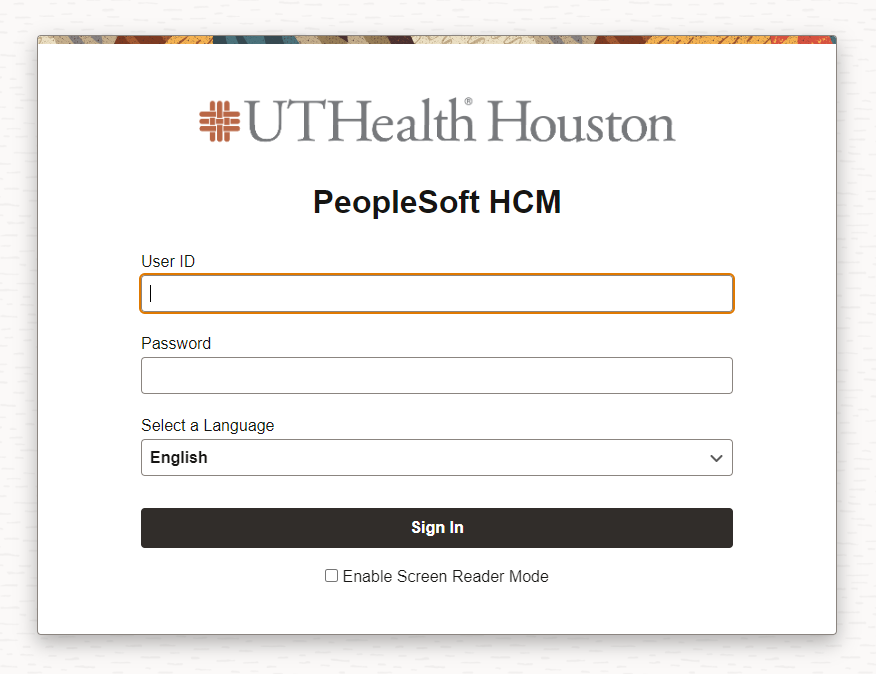
\includegraphics[width=2.92in,height=\textheight]{chapters/../graphics/self_service_login.png}
\end{center}

\begin{enumerate}
\def\labelenumi{\arabic{enumi}.}
\setcounter{enumi}{3}
\tightlist
\item
  On the next screen, click on the \texttt{Time} button.
\end{enumerate}

\begin{center}
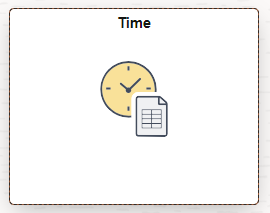
\includegraphics[width=0.9in,height=\textheight]{chapters/../graphics/time.png}
\end{center}

\begin{enumerate}
\def\labelenumi{\arabic{enumi}.}
\setcounter{enumi}{4}
\tightlist
\item
  And then the \texttt{Timesheet} button.
\end{enumerate}

\begin{center}
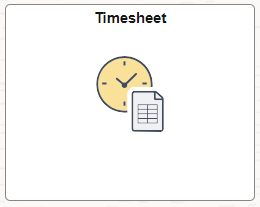
\includegraphics[width=0.87in,height=\textheight]{chapters/../graphics/timesheet_button.png}
\end{center}

\begin{enumerate}
\def\labelenumi{\arabic{enumi}.}
\setcounter{enumi}{5}
\tightlist
\item
  Finally, fill in your electronic timesheet. After your hours are
  entered, the program manager will approve them in the system, and you
  will get paid.
\end{enumerate}

\begin{center}
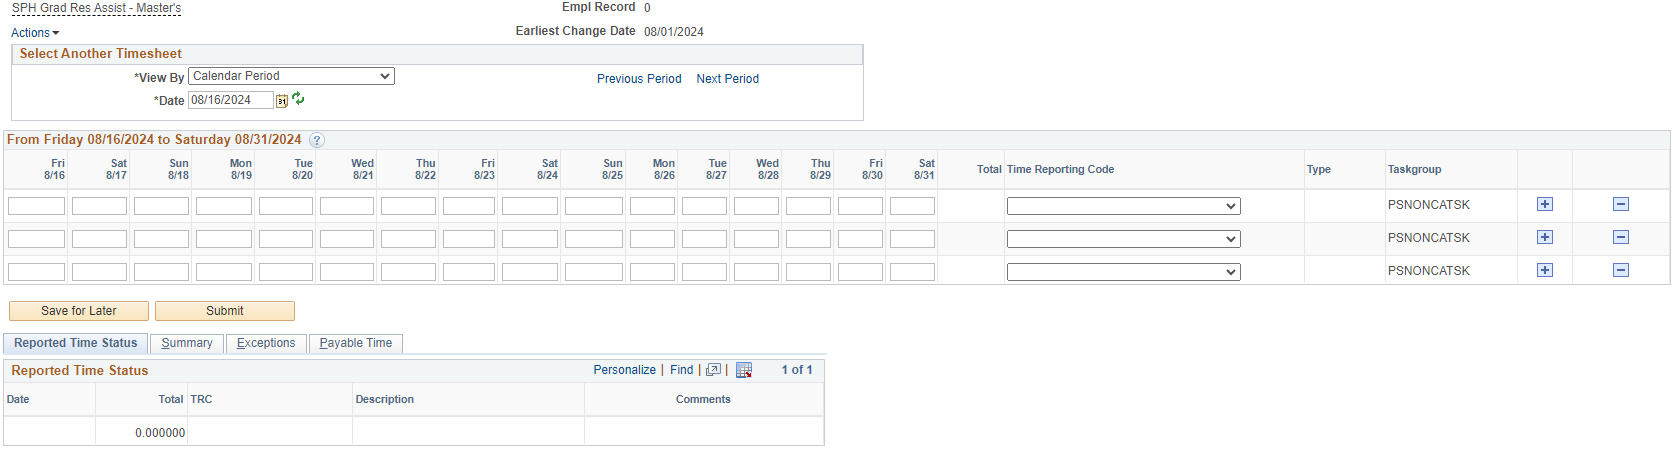
\includegraphics[width=5.58in,height=\textheight]{chapters/../graphics/timesheet.png}
\end{center}

To access W-2 forms, payroll calendars and more, click the
\texttt{Payroll\ Resources} button.

\begin{center}
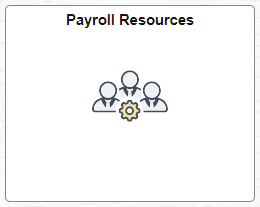
\includegraphics[width=0.87in,height=\textheight]{chapters/../graphics/payroll_resources.png}
\end{center}

If you have issues with any step in this process, you may reach out to
the IT help desk at \href{tel:7134864848}{713-486-4848}.

\section{IRB Requirements}\label{irb-requirements}

IRB stands for Institutional Review Board, and operating the IRB is one
of the most important functions of our school's Committee for the
Protection of Human Subjects. As you might have guessed from the name,
the IRB exists to review all research the school plans to conduct and
make sure that it is in compliance with all federal, state, and ethical
guidelines intended to protect human research participants.

One of the first things we will need to do when you join the team is add
you to our IRB protocols. If you haven't already done so, we will need
you to complete two steps before we can add you:

\subsection{Complete CITI training}\label{complete-citi-training}

CITI is a program that provides human subjects protection training to
many universities across the country. To complete your CITI training:

\begin{enumerate}
\def\labelenumi{\arabic{enumi}.}
\tightlist
\item
  Follow the instructions on the
  \href{https://www.uth.edu/cphs/for-researchers/training.htm\#CITI}{UTHealth
  IRB website} to log on to CITI and register.
\item
  After registering, complete the course called, ``GCP -- Social and
  Behavioral Research Best Practices for Clinical Research.''
\item
  Download the Certificate of Completion to send to the study PI and
  program manager so that they may add you to the IRB.
\end{enumerate}

\subsection{Complete Conflict of Interest (COI)
Disclosure}\label{complete-conflict-of-interest-coi-disclosure}

Every UTHealth student, staff, and faculty member who participates in
research needs to complete a COI annually. Please fill out your COI on
the \href{https://inside.uth.edu/coi/financial-disclosures.htm}{UTHealth
COI website}. You will also be able to look up frequently asked
questions while you are there. Students very rarely have any financial
conflicts of interest that they need to report, but feel free to reach
out to \href{mailto:Michael.B.Cannell@uth.tmc.edu}{Dr.~Cannell} if you
have any concerns.

\part{GRA Tasks}

\chapter{IRB Tasks}\label{sec-irb}

\subsection{IRB Documents}\label{irb-documents}

Local copies of all IRB documents for the DETECT project are located in
our SharePoint Document Library at
\href{https://uthtmc.sharepoint.com/sites/SPHDETECT-RPC/Shared\%20Documents/Forms/AllItems.aspx?FolderCTID=0x0120004E8A92AA55795C42852C8A438D043D68&id=\%2Fsites\%2FSPHDETECT\%2DRPC\%2FShared\%20Documents\%2FDETECT\%2DRPC\%20R61\%20R33\%202022\%2FIRB\%20Private}{Documents/General/IRB
Private}. You may need to read, copy, and/or update these files from
time to time.

\subsection{iRIS}\label{iris}

Virtually all IRB documentation will be submitted and stored in
\href{https://iris.uth.tmc.edu/}{UTHealth's Integrated Research
Information Software (iRIS)}. If you have iRIS-related questions, you
may contact the iRIS help line at \href{tel:7135007960}{713-500-7960}.

As part of your responsibilities as a GRA, you may or may not be asked
to directly create or edit research protocols/documents in the iRIS
system. After you sign in, you will land on the iRIS home screen. There
can be multiple sections and studies listed on your iRIS home screen,
but there should be a little pencil and paper icon on the left-hand side
of every active study and study update that you have access to. Here is
an example from Dr.~Cannell's iRIS home screen with the pencil and paper
icon highlighted in red.

\begin{center}
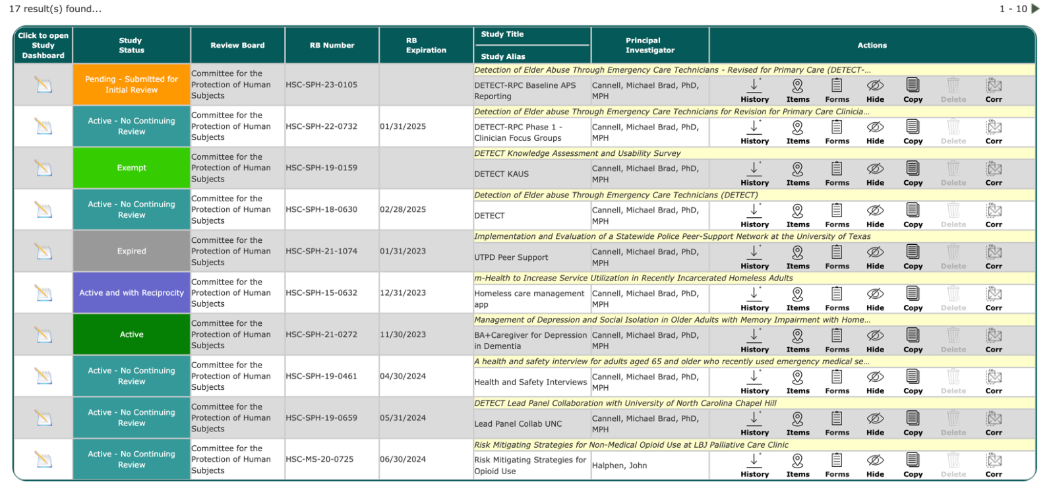
\includegraphics[width=3.49in,height=\textheight]{chapters/gra_tasks/../../graphics/iris.png}
\end{center}

\subsection{IRB Change Requests and
Amendments}\label{irb-change-requests-and-amendments}

One task that we commonly ask GRA's to assist us with is submitting
change requests and amendments. Change requests and amendments are
typically used to let the IRB know that we intend to change something
about the way we are conducting our study. For example, if we originally
told the IRB that we would pay research participants \$20 and we later
decide to pay them \$25, then we will need to submit that change to the
IRB for approval.

To access a change request form, click on the pencil and paper icon for
the study you are working on. The next screen should look something like
this.

\begin{center}
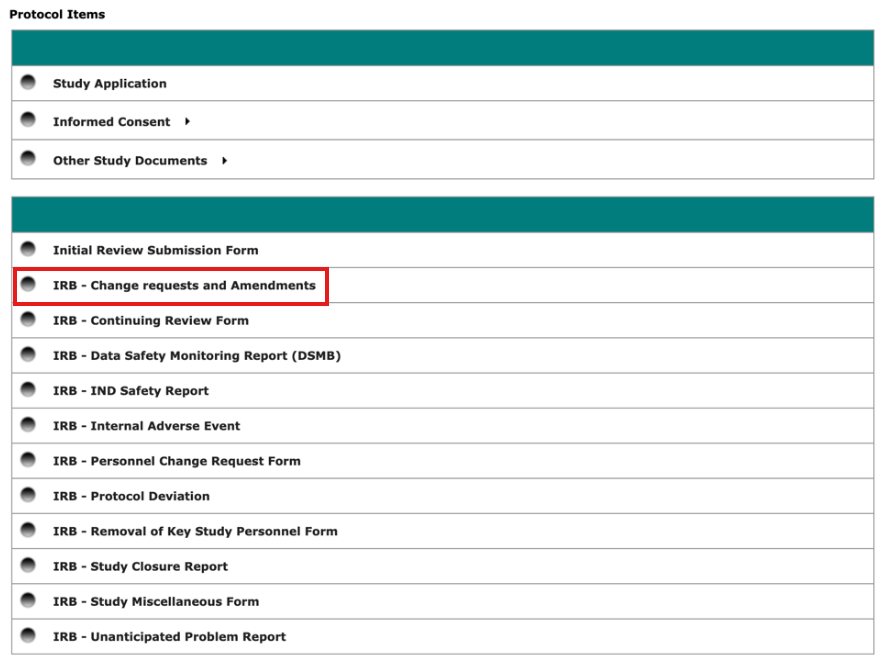
\includegraphics[width=2.94in,height=\textheight]{chapters/gra_tasks/../../graphics/change_request.png}
\end{center}

One of the options will be
\texttt{IRB\ –\ Change\ requests\ and\ Amendments} -- click it. On the
next page, click the \texttt{Add\ a\ New\ Form} button. Each protocol is
somewhat unique, so it's difficult to provide instructions on precisely
what to type into the form. However, here are some notes that previous
GRAs found useful about the DETECT project specifically. Please keep in
mind that we can change any part of the form before our final
submission.

\begin{itemize}
\tightlist
\item
  Update number: If this is the first protocol update, then the update
  number will be 1. If it's the second, then 2, and so on.
\item
  Short description. Just do your best to write something succinct and
  descriptive.
\item
  Does the revision to this protocol require a formal change to the
  title: Typically, not.\\
\item
  Memorial Hermann location questions: Typically, the answer to all of
  these is ``No.''
\item
  Type of revisions: Select those that seem applicable.
\item
  Revision description and rationale: What changes do we want to make
  and why do we want to make them?
\item
  Who is initiating this change: Typically, Investigator-initiated.
\item
  Risk increase: Typically, the revision will not increase risk to
  participants.
\item
  Designated Department Approval/Head: Bijal Bala.
\item
  Funding: DETECT is federally funded by the National Institutes of
  Health (NIH) and the National Institute on Aging (NIA).
\end{itemize}

It can often be helpful to start by looking at other change requests
that have been submitted and approved. At the end of the day, we ask
that you just fill out the form(s) to the best of your ability. When you
are done, please email the PI and program manager to let them know. They
will review all of the forms and likely make edits before the final
submission.

\subsection{IRB Personnel Change
Requests}\label{irb-personnel-change-requests}

Another common task we ask GRAs to help with is adding or removing
personnel from the study.

To access a personnel change request form, click on the pencil and paper
icon for the study you are working on. The next screen should look
something like this.

\begin{center}
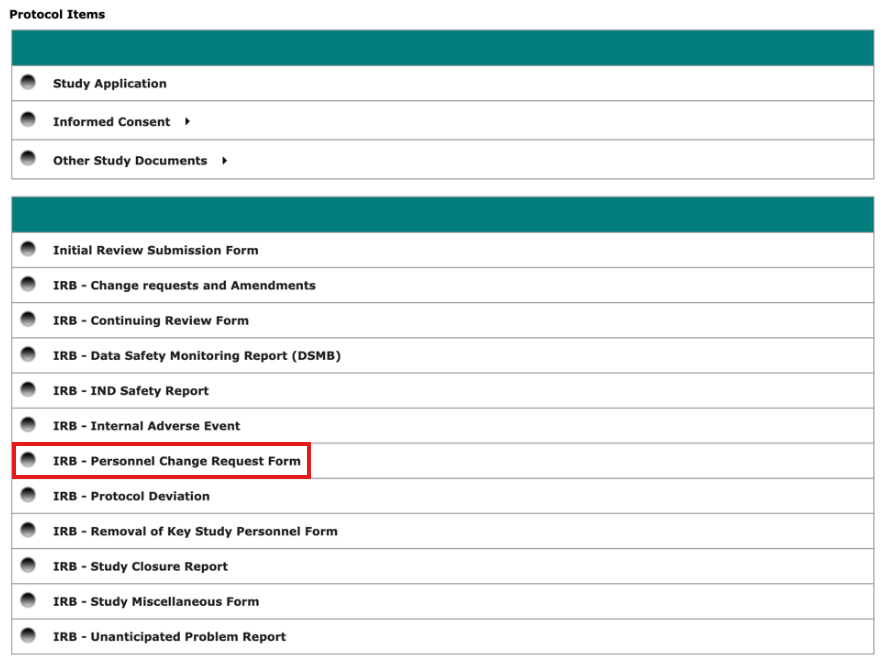
\includegraphics[width=2.94in,height=\textheight]{chapters/gra_tasks/../../graphics/personnel_change.png}
\end{center}

One of the options will be
\texttt{IRB\ –\ Personnel\ Change\ Request\ Form} -- click it. On the
next page, click the \texttt{Add\ a\ New\ Form} button. Here are some
notes for filling out the form that previous GRAs found useful. Please
keep in mind that we can change any part of the form before our final
submission.

\begin{itemize}
\tightlist
\item
  Are you requesting a change to the principal investigator: No.~
\item
  Are you requesting the addition of a co-investigator: Maybe. Ask the
  PI or Program Manager if you are unsure.
\item
  Are you requesting changes to key study personnel: This is the most
  common scenario.
\item
  To add co-investigators or key personnel, we will need to have their
  CITI certificate and they will have to complete a COI. Both of these
  documents are explained above.
\item
  Are you removing anyone from the study at this time: If we are, please
  just write their name and a brief explanation. For example, ``Jane
  Smith. She graduated in May.''
\item
  Typically, we prefer not to add and remove personnel on the same form.
  So, if we need to add Jon Smith to the protocol and we need to remove
  Jane Smith from the protocol, we should do so using two separate
  forms.
\item
  Significant financial interest: This is almost always ``No.'' So,
  please select ``No.'' The PI will change it to ``Yes'' before the
  final submission if necessary.
\item
  Additional information: You can leave this blank.
\item
  Designated Department Approval/Head: Bijal Bala.
\item
  Funding: DETECT is federally funded by the National Institutes of
  Health (NIH) and the National Institute on Aging (NIA).
\end{itemize}

At the end of the day, we ask that you just fill out the form(s) to the
best of your ability. When you are done, please email the PI and program
manager to let them know. They will review all of the forms and likely
make edits before the final submission.

\chapter{Data Management and Analysis Tasks}\label{sec-data}

Most, if not all, of our research projects will involve the management
and analysis of data. This section of the SOP includes information
intended to make it easier for us to find and use the files we need to
access, manage, and analyze project data. These files broadly include
project data files, programming code files, and general project
documentation files. All three will be covered below. However, there are
a couple of general topics that we should familiarize ourselves with
first. Namely, protective health information (PHI), reproducible
research, and GitHub.

\subsection{Protected Health
Information}\label{protected-health-information}

We should already be familiar with PHI from our
\href{https://www.uth.edu/cphs/for-researchers/training.htm}{CITI
training courses}. However, this concept is so important that it bears
repeating here. The UC Berkely Human Research Protection Program website
summarizes PHI this way:

\begin{quote}
\emph{Protected Health Information (PHI) is any information in the
medical record or designated record set that can be used to identify an
individual and that was created, used, or disclosed in the course of
providing a health care service such as diagnosis or treatment. HIPAA
regulations allow researchers to access and use PHI when necessary to
conduct research. However, HIPAA applies only to research that uses,
creates, or discloses PHI that enters the medical record or is used for
healthcare services, such as treatment, payment, or operations}.
\end{quote}

It further goes on to list 18 identifiers that can be used to identify
the individual associated with the health records. They are:

\begin{enumerate}
\def\labelenumi{\arabic{enumi}.}
\tightlist
\item
  Names;
\item
  All geographical subdivisions smaller than a State, including street
  address, city, county, precinct, zip code, and their equivalent
  geocodes, except for the initial three digits of a zip code, if
  according to the current publicly available data from the Bureau of
  the Census: (1) The geographic unit formed by combining all zip codes
  with the same three initial digits contains more than 20,000 people;
  and (2) The initial three digits of a zip code for all such geographic
  units containing 20,000 or fewer people is changed to 000.
\item
  All elements of dates (except year) for dates directly related to an
  individual, including birth date, admission date, discharge date, date
  of death; and all ages over 89 and all elements of dates (including
  year) indicative of such age, except that such ages and elements may
  be aggregated into a single category of age 90 or older;
\item
  Phone numbers;
\item
  Fax numbers;
\item
  Electronic mail addresses;
\item
  Social Security numbers (SSN);
\item
  Medical record numbers (MRN);
\item
  Health plan beneficiary numbers;
\item
  Account numbers;
\item
  Certificate/license numbers;
\item
  Vehicle identifiers and serial numbers, including license plate
  numbers;
\item
  Device identifiers and serial numbers;
\item
  Web Universal Resource Locators (URLs);
\item
  Internet Protocol (IP) address numbers;
\item
  Biometric identifiers, including finger and voice prints;
\item
  Full face photographic images and any comparable images; and
\item
  Any other unique identifying number, characteristic, or code (note
  this does not mean the unique code assigned by the investigator to
  code the data)
\end{enumerate}

\subsection{Reproducible Research}\label{reproducible-research}

We will strive to make our projects conform to best practices for
promoting reproducible research. Many resources that describe what
reproducible research is, and why it's important, are available on the
internet, and we encourage you to look at some of them. Briefly, here is
an excerpt from
\href{https://en.wikipedia.org/wiki/Reproducibility}{Wikipedia} that is
good enough for our purposes:

\begin{quote}
\emph{``The term reproducible research refers to the idea that
scientific results should be documented in such a way that their
deduction is fully transparent. This requires a detailed description of
the methods used to obtain the data and making the full data set and the
code to calculate the results easily accessible. This is the essential
part of open science.}

\emph{To make any research project computationally reproducible, general
practice involves all data and files being clearly separated, labelled,
and documented. All operations should be fully documented and automated
as much as practicable, avoiding manual intervention where feasible. The
workflow should be designed as a sequence of smaller steps that are
combined so that the intermediate outputs from one step directly feed as
inputs into the next step. Version control should be used as it lets the
history of the project be easily reviewed and allows for the documenting
and tracking of changes in a transparent manner.''}
\end{quote}

Because the data we work with almost always includes (PHI), we will not
typically be able to make our data freely available to the general
public. However, we will do our best to conform to the remaining
elements of reproducible research described above. Two of the most
important tools we will use to make our research more reproducible are
\href{https://git-scm.com/}{git} and \href{https://github.com/}{GitHub}.

\subsubsection{GitHub}\label{github}

\href{https://github.com/}{GitHub} is a website specifically designed to
facilitate collaboratively creating programming code. In many ways,
GitHub is a cloud-based file storage service like Dropbox, Google Drive,
or OneDrive. However, GitHub contains some additional features that make
it an exceptional tool for collaborating our research projects. Some of
these features include:

\begin{itemize}
\tightlist
\item
  Repositories
\item
  Projects
\item
  Discussions
\item
  Wikis
\end{itemize}

\paragraph{GitHub Repositories}\label{github-repositories}

We will make extensive use of \href{https://github.com/}{GitHub}
repositories. If you aren't already familiar with git and GitHub, please
start by reading the relevant chapters in
\href{https://www.r4epi.com/introduction-to-git-and-github.html}{R for
Epidemiology}. It's probably a good idea to read those chapters even if
you are already familiar with git and GitHub because they describe how
we will use our GitHub repositories. Here are some key summary points to
keep in mind:

\begin{itemize}
\tightlist
\item
  Almost all programming code, code documentation, and even a large
  amount of general project documentation will flow through our
  projects' GitHub repositories.
\item
  Almost all of our programming tasks will be tracked using GitHub
  projects.
\item
  Please work with the project PI and/or program manager to make sure
  you are able to locate and access the GitHub repositories and GitHub
  project(s) associated with the research project(s) you are working on.
\end{itemize}

\paragraph{GitHub Projects}\label{github-projects}

GitHub projects -- we will sometimes refer to them as project boards --
allow us to organize, track, and communicate about
\href{https://docs.github.com/en/issues/tracking-your-work-with-issues/about-issues}{GitHub
issues}. The name ``issues'' sort of implies a problem, but that isn't
how we will use them. We will use issues as tasks that need to be
completed, and we will use project boards to track those tasks. In fact,
for the rest of this continuity guide, I will refer to them as tasks
instead of issues.

\begin{center}
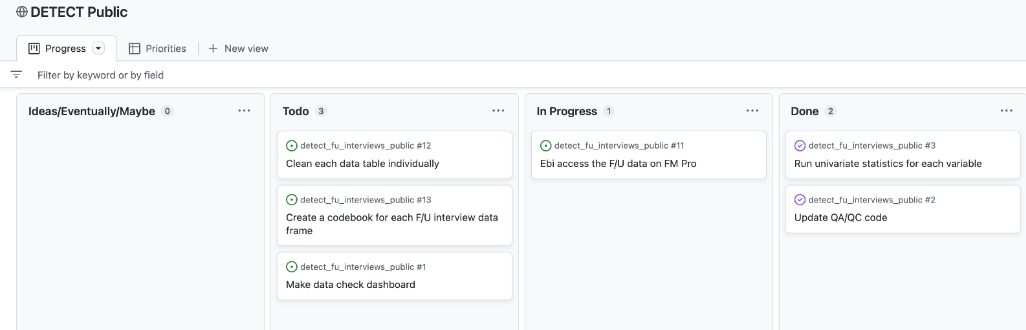
\includegraphics[width=3.42in,height=\textheight]{chapters/gra_tasks/../../graphics/project.png}
\end{center}

The example above is from the DETECT project and we can see examples of
tasks that are yet to be started (i.e., Ideas/Eventually/Maybe and
Todo), in progress, and already completed (i.e., Done). We can click on
the tasks to open a detailed view where we can add a description, we can
add sub tasks, and we can leave messages for each other about the task.

There are a couple of advantages to messaging each other about tasks in
GitHub instead of sending emails. First, the messages stay with the
tasks they are about. You don't have to go search for them later, and
all the information/context you need is in one place. Second, when you
graduate and leave UTHealth, your email account will be deleted.
However, that doesn't necessarily mean you will want to quit working on
a project. Fortunately, if we've been communicating in GitHub instead of
through email, nothing important is lost.

\paragraph{GitHub Discussions}\label{github-discussions}

\begin{center}
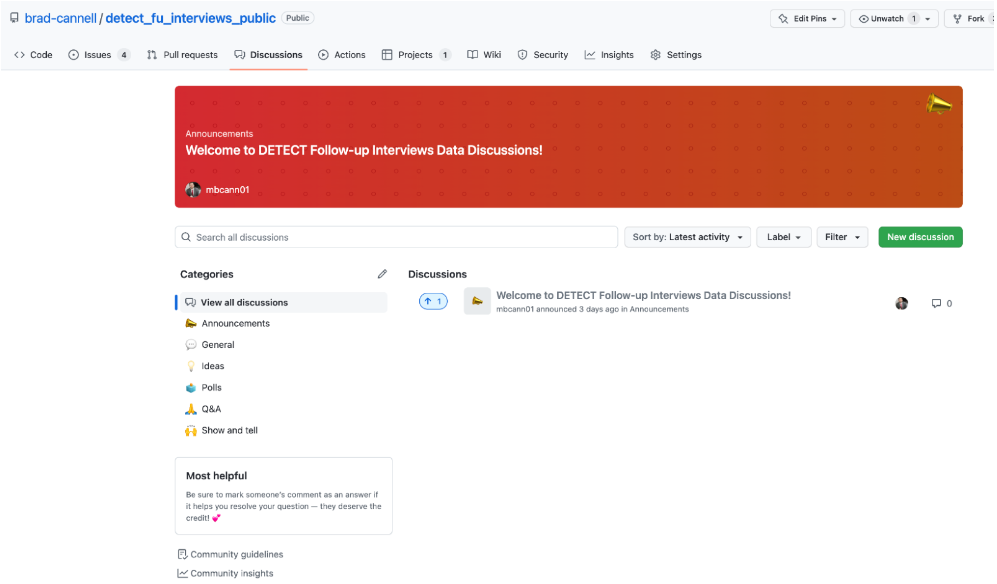
\includegraphics[width=3.32in,height=\textheight]{chapters/gra_tasks/../../graphics/discussions.png}
\end{center}

As the name indicates, GitHub discussions are a place where we can have
discussions about the project. For example, we can exchange ideas and we
can ask each other general questions that don't necessarily pertain to a
specific task.

\paragraph{GitHub Wikis}\label{github-wikis}

\begin{center}
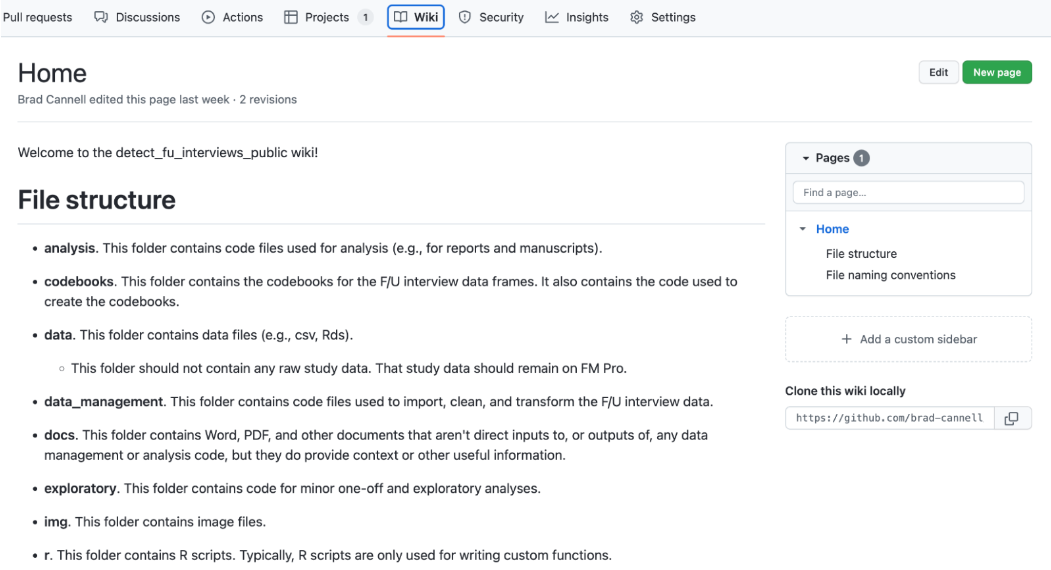
\includegraphics[width=3.5in,height=\textheight]{chapters/gra_tasks/../../graphics/wikis.png}
\end{center}

We can generally think of GitHub wikis as an SOP for a specific
repository. Wikis aren't about what to do -- that's what tasks are for.
Rather, wikis tend to contain information about how to navigate and use
the repository and how to complete our tasks in a consistent way. For
example, the screenshot above shows part of the
\href{https://github.com/brad-cannell/detect_fu_interviews_public/wiki}{DETECT
follow-up interview repository's wiki}. In this particular screenshot,
we can see instructions for navigating and using the repository's
file/folder structure.

\subsubsection{Communicating About Research
Projects}\label{communicating-about-research-projects}

Over time, I have come to really appreciate the number and quality of
tools that GitHub provides for collaboratively coding and working on
research projects. It truly is an amazing tool in my opinion. Having
said that, I understand how it can be pretty intimidating -- or at least
overwhelming -- at first. So, here is a little cheat sheet to get us
started.

\begin{center}
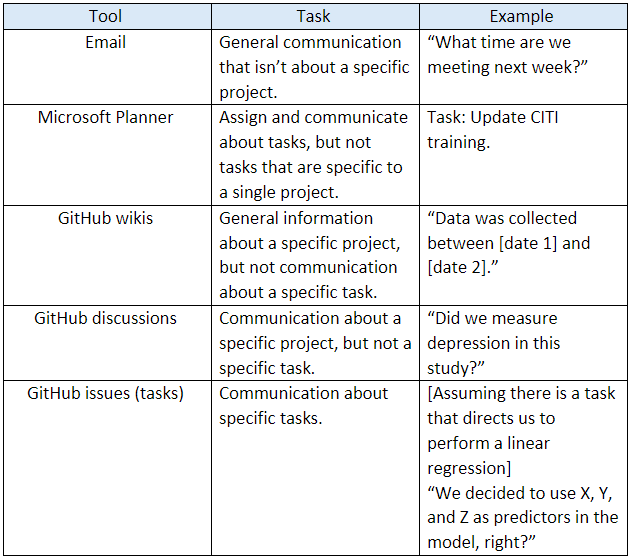
\includegraphics[width=0.75\textwidth,height=\textheight]{chapters/gra_tasks/../../graphics/cheat_sheet.png}
\end{center}

Here are some additional notes about communication to keep in mind:

\begin{itemize}
\tightlist
\item
  Please follow the guidance in R4Epi when you have a coding question.
\item
  When creating commits, please follow the guidance in R4Epi.

  \begin{itemize}
  \tightlist
  \item
    Scroll down to the paragraph that begins with, ``The first line is
    called the commit message.''
  \end{itemize}
\end{itemize}

\subsubsection{Separation of Data and
Code}\label{separation-of-data-and-code}

By design, public GitHub repositories are not secure -- they are
publicly available. So, why do we use them? As discussed above, we use
them because we want our research to be as transparent and reproducible
as possible. Having said that, we have an obligation to balance
reproducibility with the protection of the participants who make our
research possible. Our best effort at striking that balance will be to
upload almost everything {except data} to our GitHub repositories and
make it publicly available. Other people will still be able to use the
data, but they will need to follow certain procedures.

We believe the reproducible research approach is the most ethical and
productive way to conduct research; however, it does create some
additional complications for us. Namely, we can't store the data in our
code repository, but we still want to use relative file paths in our
code (Please read \href{https://www.r4epi.com/r-projects.html}{this
chapter in R4Epi} if you aren't familiar with the difference between
relative and absolute file paths). In other words, the file paths we use
in the code should work on team member's computer without having to make
any alterations to it. There are at least a couple of different ways we
can accomplish this.

\begin{enumerate}
\def\labelenumi{\arabic{enumi}.}
\tightlist
\item
  Create a \texttt{data} folder in the repository, but make sure to
  \href{https://www.r4epi.com/using-git-and-github.html\#step-4-update-and-commit-gitignore}{gitignore}
  all of the data files in the data folder. a. We will then exchange
  data to add to the folder using a process that is separate from
  cloning the repository. For example, we will exchange the data using a
  shared OneDrive folder, you will copy the data from the shared
  OneDrive folder into the \texttt{data} folder in your local
  repository.
\item
  Another option that is sometimes available is to store the data in a
  remote database (e.g., FileMaker Pro). Then, we connect to the data
  using ODBC. a. When using this method, we have to make sure we don't
  add our database username and password to the code that will be
  publicly available on GitHub. Additionally, we need to make sure that
  the code we use to access the remote database is identical on every
  team member's computer. A credential storage application like
  \href{https://github.com/r-lib/keyring}{Keyring} helps us meet both of
  these needs.
\end{enumerate}

What if we do accidentally upload data, PHI, or passwords? Don't freak
out! Just let the PI know and we will fix it together.

\subsubsection{Writing Programming Code}\label{writing-programming-code}

When writing programming code we generally will follow the guidance
given in the \href{https://www.r4epi.com/r-scripts.html}{coding tools
and best practices part of R4Epi}. If you haven't already done so,
please go ahead and read those chapters. In addition to reading about
the coding style we will use, there are a couple of R packages that can
help you style your code. They are
\href{https://lintr.r-lib.org/}{lintr} and
\href{https://styler.r-lib.org/}{styler}. We highly recommend that you
give them a try.

Here are some additional guidelines that may not jump out at you.

\begin{itemize}
\tightlist
\item
  Use \href{https://quarto.org/}{Quarto} documents.

  \begin{itemize}
  \tightlist
  \item
    \href{https://www.r4epi.com/quarto-files}{Click here to read about
    Quarto files in R for Epidemiology}.
  \item
    We will almost always write our code in Quarto documents (as opposed
    to R scripts). However, we generally don't need to render them into
    HTML, Word, or PDF documents. The exception to this guideline
    includes:

    \begin{itemize}
    \tightlist
    \item
      We will typically write functions in R scripts when they will be
      used in more than one Quarto file.
    \item
      We will write Shiny applications in R scripts.
    \item
      If the project we are working on is an R package (as opposed to a
      research project), all functions will be written in R scripts.
    \end{itemize}
  \end{itemize}
\item
  Don't add dates or your name to code files. That is what versioning is
  for.

  \begin{itemize}
  \tightlist
  \item
    \textbf{Do this:} \texttt{01\_data\_import}.
  \item
    \textbf{Do not do this:} \texttt{01\_data\_import\_mbc\_edits},
    \texttt{01\_data\_import\_v2},
    \texttt{01\_data\_import\_2023\_06\_14}.
  \end{itemize}
\end{itemize}

\subsubsection{Getting Started Task
List}\label{getting-started-task-list}

Now that you have some basic information about our team process for
working on data management and analysis, here is a quick task list to
get you started. It should be applicable for just about any project you
are working on.

\begin{itemize}
\tightlist
\item
  Make sure you've read the most applicable sections of R4Epi. Please
  pay special attention to:

  \begin{itemize}
  \tightlist
  \item
    The \href{https://www.r4epi.com/asking-questions.html}{chapter on
    asking questions}.
  \item
    All of the \href{https://www.r4epi.com/r-scripts.html}{chapters in
    the coding tools and best practices part} of the book.
  \item
    All of the
    \href{https://www.r4epi.com/introduction-to-git-and-github.html}{chapters
    on using git and GitHub}.
  \end{itemize}
\item
  Make sure you have already been added to the IRB protocol.
\item
  Download all necessary software to your computer (e.g., RStudio, git,
  FM pro driver, GitKraken).
\item
  Create all necessary subscriptions (e.g., GitHub).
\item
  Fork the GitHub repository to your GitHub account.
\item
  Clone the GitHub repository to your computer.
\item
  Create a test pull request.
\item
  Make sure you can access any data needed for the project.
\item
  Start looking through the tasks on the GitHub project board.
\end{itemize}

\part{Style Guide}

\section*{Overview}\label{sec-sg_overview}
\addcontentsline{toc}{section}{Overview}

\markright{Overview}

The ultimate goal of a style guide is to reduce cognitive load. Doing so
should improve the quality and consistency of our work product and make
our work lives easier and more efficient. How does a style guide do
this?

\begin{itemize}
\item
  First, it reduces the number of choices we need to make as we are
  authoring content. For example, we don't need to come up with our own
  answers to questions like, ``where should I put this document?'' or
  ``what should I name this folder?''
\item
  Second, having the predetermined choices written down for reference
  reduces the amount of information we need to store in our intentional
  memory. For example, ``OK, remember to always start these file names
  with the date written as yyyy-mm-dd''. Although we don't need to
  \emph{intentionally} memorize them, these predetermined choices may
  eventually bleed over into our memory by accident through repetition.
\item
  Third, having uniformly styled content makes it easier for others --
  \emph{including future us} -- to find what we are looking for and use
  it. We can focus our brain power on the content instead of the style
  and/or organization of the content.
\end{itemize}

\chapter{Emphasizing Text}\label{sec-emph_text}

Use the following conventions to emphasize keywords, concepts, code
snippets, and other words or phrases that need to stand out or be
emphasized.

\subsection{Application Names}\label{application-names}

Capitalize the names of applications.

\begin{itemize}
\tightlist
\item
  Do this: Microsoft Outlook, Outlook, Microsoft Planner, Planner.
\item
  Do not do this: microsoft outlook, outlook, microsoft planner,
  planner.
\end{itemize}

\subsection{Keywords}\label{keywords}

Underline a keyword or phrase if it is a keyword or phrase that we would
want to define in the glossary of the document (whether the document
actually has a glossary or not).

\begin{itemize}
\tightlist
\item
  \textbf{Do this:} \ul{A standard operating procedure} (SOP) is\ldots{}
\item
  \textbf{Do not do this: A standard operating procedure (SOP)}
  is\ldots, A standard operating procedure (SOP) is\ldots{}
\end{itemize}

\textbf{Bold} a keyword or phrase that we want to call attention to, but
it is not necessarily a keyword or phrase that we would want to define
in the glossary of the document (whether the document actually has a
glossary or not).

\begin{itemize}
\tightlist
\item
  \textbf{Do this:} **Step 1.**, ** Do this:**.
\item
  \textbf{Do not do this:} \ul{Step 1.}, Do this.
\end{itemize}

At times, we will also \emph{Italicize} keywords or phrases that we want
to call attention to, but are not necessarily keywords or phrases that
we would want to define in the glossary of the document (whether the
document actually has a glossary or not). In general, we will follow
\href{https://www.grammarly.com/blog/italics/}{standard English grammar
rules for using the italics typeface} (pay special attention to bullet
14). Further, ``avoid using italics with other stylized typefaces, such
as bold and underline. Since all three are designed to make words stand
out, only one at a time is necessary.''
(\href{https://www.grammarly.com/blog/italics/}{Ellis, 2022})

\begin{itemize}
\tightlist
\item
  \textbf{Do this:} We do not want to coerce participants into signing
  the consent form.
\item
  \textbf{Do not do this:} We do
  NOT/\textbf{not}/\emph{not}/\textbf{\emph{not}}/\ul{\textbf{\emph{not}}}
  want to coerce participants into signing the consent form.
\end{itemize}

\subsection{Programming Code}\label{programming-code}

Snippets of programming code should be written in the
\texttt{Courier\ New} font with a light gray background. This matches
the style convention used by many popular programming websites like
GitHub and Stack Overflow. To make using this format easier, any
document that was created by duplicating the New SOP Template will have
a \texttt{code} option in the styles menu.

\begin{center}
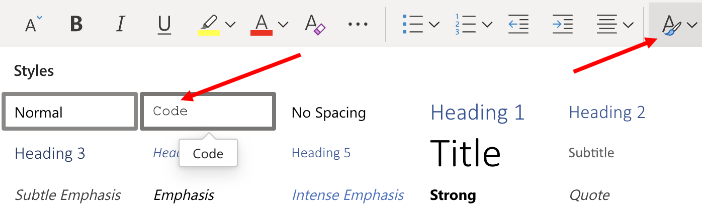
\includegraphics[width=2.34in,height=\textheight]{chapters/style_guide/../../graphics/code_snippet.png}
\end{center}

\begin{itemize}
\tightlist
\item
  \textbf{Do this:} \texttt{utcNow()}, \texttt{dplyr::select()}.
\item
  \textbf{Do not do this:} utcNow(), \emph{dplyr::select()},
  \textbf{dplyr::select()}, ``dplyr::select()''
\end{itemize}

\subsection{Clickable Operations in
Applications}\label{clickable-operations-in-applications}

In many of the applications we use, clickable steps or operations serve
the same function as programming code. For example, in Microsoft word,
we don't type ``bold(`Do this')''. Instead, we highlight the phrase ``Do
this'' with our mouse and then click the \texttt{B} button in the
toolbar. Then, Microsoft Word takes care of the programming behind the
scenes for us. Therefore, clickable operations that need to be performed
in an application should be written in same style used to write code. To
make using this format easier, any document that was created by
duplicating the New SOP Template will have a \texttt{code} option in the
styles menu.

\begin{itemize}
\tightlist
\item
  \textbf{Do this:} Click on the \texttt{Insert} tab\ldots{}
\item
  \textbf{Do not do this:} Click on the
  \emph{Insert}/INSERT/\textbf{insert}/\ul{insert} tab.
\end{itemize}

\subsection{File Paths}\label{file-paths}

All file paths should be written in italic text with a light gray
background. To make using this format easier, any document that was
created by duplicating the New SOP Template will have a
\texttt{File\ Paths} option in the styles menu. Additionally, the root
directory (i.e., starting point) for all SharePoint/Teams documents is
the Documents folder.

\begin{itemize}
\tightlist
\item
  \textbf{Do this:}
  \texttt{Documents/General/SOPs/02\ Style\ Guide.docx}.
\item
  \textbf{Do not do this:} ``Documents/General/SOPs/02 Style
  Guide.docx''.
\end{itemize}

\subsection{File and Folder Names}\label{file-and-folder-names}

File and Folder names are essentially very short file paths. Therefore,
file names and folder names should be written using the file paths
guidelines from above. There is one exception to this rule. When
creating a hyperlink to a file or folder, then the standard hyperlink
style (i.e., \href{}{link}) should be used.

\begin{itemize}
\tightlist
\item
  \textbf{Do this:} The \texttt{SOP} folder.
\item
  \textbf{Do not do this:} The ``SOP'' folder. The \textbf{SOP} folder.
\end{itemize}

\chapter{Document Library Structure}\label{sec-doc_lib_structure}

\subsection{Folder Structure}\label{folder-structure}

\begin{itemize}
\tightlist
\item
  Each folder in the document library should generally be associated
  with a specific theme or topic, which may have sub-themes and
  subtopics.

  \begin{itemize}
  \tightlist
  \item
    \textbf{Do this:} \texttt{IRB\ Documents} or
    \texttt{Budget\ Documents}.
  \item
    \textbf{Do not do this:} \texttt{Budgets\ and\ IRB\ Documents}.
  \end{itemize}
\item
  Folders should not generally be associated with specific people or
  positions. There are at least two reasons why we don't want to
  associate folders with people or positions. First, people and
  positions change over time. Topics can change too, but they tend to be
  more stable. Second, and perhaps more importantly, this is a shared
  document library. We shouldn't think of anything we keep in this
  library as belonging to any individual. As such, the names and
  purposes of documents should be clear to others who may need to use
  them. For example, it's going to be much easier for most people to
  reason about what is contained in the \texttt{IRB} folder than in the
  \texttt{Brad} folder.

  \begin{itemize}
  \tightlist
  \item
    \textbf{Do this:} \texttt{IRB\ Documents} or
    \texttt{Budget\ Documents}.
  \item
    \textbf{Do not do this:} \texttt{Brad’s\ Documents} or
    \texttt{GRA\ Documents}.
  \end{itemize}
\item
  Folders that can be logically nested inside an existing folder, or two
  similar folders that can logically be combined under a single parent
  folder, should be.

  \begin{itemize}
  \tightlist
  \item
    For example, a folder containing CITI training certificates should
    probably be nested in the \texttt{IRB\ Documents\ folder}.\\
  \item
    A folder containing GRA applicant resumes, a folder containing GRA
    work schedules, and a folder containing job announcements should
    probably all be nested in a \texttt{Hiring} folder, which should
    probably be nested in a \texttt{HR} folder.
  \end{itemize}
\end{itemize}

\subsection{Folder Names}\label{folder-names}

\begin{itemize}
\tightlist
\item
  Folders for programming code repositories should be written in snake
  case. This is to help ensure that the folder name works easily with R,
  Git, Bash, and other software used in the data analysis pipeline.

  \begin{itemize}
  \tightlist
  \item
    \textbf{Do this:} \texttt{detect\_public\_repo}.
  \item
    \textbf{Do not do this:} \texttt{DETECT\ Public\ Repo}.
  \end{itemize}
\item
  All other folders should be written in title case.

  \begin{itemize}
  \tightlist
  \item
    \textbf{Do this:} \texttt{Budget\ Documents}.
  \item
    \textbf{Do not do this:} \texttt{budget\ documents}.
  \end{itemize}
\item
  Folder names should be descriptive enough for most people to
  reasonably be able to figure out what the folder contains from the
  name.

  \begin{itemize}
  \tightlist
  \item
    \textbf{Do this:} \texttt{Budget\ Documents}.
  \item
    \textbf{Do not do this:} \texttt{Brad’s\ Stuff} or
    \texttt{MU-334-011}.
  \end{itemize}
\item
  Folder names should be succinct.

  \begin{itemize}
  \tightlist
  \item
    \textbf{Do this:} \texttt{Pre-award}.
  \item
    \textbf{Do not do this:}
    \texttt{Narrative\ –\ Spec\ Aims\ –\ Budgets\ –\ and\ Other\ Documents\ Submitted\ to\ NIA\ in\ the\ Original\ Proposal}.
  \end{itemize}
\item
  Folder names should only include letters, numbers, underscores, or
  dashes. Other characters can cause syncing failures and/or issues with
  other file systems.

  \begin{itemize}
  \tightlist
  \item
    \textbf{Do this:} \texttt{Materials\ and\ Operations}.
  \item
    \textbf{Do not do this:} \texttt{Materials\ \&\ Operations}.
  \end{itemize}
\item
  Folders that can be naturally arranged by dates should be. The folder
  name should begin with the date written in the \textbf{yyyy-mm-dd}
  format. This format is important because dates written in this format
  will naturally be arranged in correct chronological order across
  years. Some examples of folder topics that may have a natural
  chronological order include IRB documents, budgets, and meeting
  minutes.

  \begin{itemize}
  \tightlist
  \item
    \textbf{Do this:} \texttt{2023-02-17\ Budget}.
  \item
    \textbf{Do not do this:}
    \texttt{February\ Budget\ or\ 02-17-2023\ Budget}.
  \end{itemize}
\item
  Folders that can be naturally arranged in a sequential order should
  be. When doing so, the folder names should be sequentially numbered.
  Single digits should be prefixed with a zero (0). This format is
  important because single digits written in this format will naturally
  be arranged in correct sequential order when the number of folders in
  the sequence exceeds 9. Data analysis projects are an example where
  folder topics may have a natural sequential order.

  \begin{itemize}
  \tightlist
  \item
    \textbf{Do this:}
    \texttt{01\_data\_import,\ 02\_data\_clean,\ 03\_table\_01,\ 04\_table\_04}.
  \item
    \textbf{Do not do this:}
    \texttt{1\_data\_import,\ 2\_data\_clean,\ table\_1,\ my\_other\_table}.
  \end{itemize}
\item
  Folders for documents related to peer-reviewed manuscripts should
  begin with the first author's last name.

  \begin{itemize}
  \tightlist
  \item
    \textbf{Do this:} \texttt{Cannell\ –\ Protocol\ Paper}.
  \item
    \textbf{Do not do this:} \texttt{Protocol\ Paper}.
  \end{itemize}
\item
  When multiple folders have a similar theme/topic, begin the folder
  names with a description of the theme/topic. Doing so will ensure that
  all folders with that theme/topic are grouped together in the file
  list.

  \begin{itemize}
  \tightlist
  \item
    \textbf{Do this:} \texttt{Reliance\ Agreement\ UAB},
    \texttt{Reliance\ Agreement\ UCSF},
    \texttt{Reliance\ Agreement\ JHU}.
  \item
    \textbf{Do not do this:} \texttt{UAB\ Reliance\ Agreement},
    \texttt{UCSF\ Reliance\ Agreement},
    \texttt{JHU\ Reliance\ Agreement}.
  \end{itemize}
\end{itemize}

\subsection{File Structure}\label{file-structure}

\begin{itemize}
\tightlist
\item
  Files should generally be grouped together and placed in a folder that
  describes the theme or topic they belong to.
\item
  Folders that contain a single file should be rare.
\end{itemize}

\subsection{File Names}\label{file-names}

\begin{itemize}
\tightlist
\item
  Programming code files should be written in snake case. This is to
  help ensure that the file name works easily with R, Git, Bash, and
  other software used in the data analysis pipeline.

  \begin{itemize}
  \tightlist
  \item
    \textbf{Do this:} \texttt{01\_data\_import.Rmd}.
  \item
    \textbf{Do not do this:} \texttt{Data\ Import.Rmd}.
  \end{itemize}
\item
  All other file names should be written in title case.

  \begin{itemize}
  \tightlist
  \item
    \textbf{Do this:} \texttt{Cannell\ CITI\ Certificate.pdf}.
  \item
    \textbf{Do not do this:} \texttt{cannell\ citi\ certificate.pdf}.
  \end{itemize}
\item
  File names should be descriptive enough for most people to reasonably
  be able to figure out what the file contains from the name.

  \begin{itemize}
  \tightlist
  \item
    \textbf{Do this:} \texttt{Cannell\ CITI\ Certificate.pdf}.
  \item
    \textbf{Do not do this:} \texttt{CITI.pdf}.
  \end{itemize}
\item
  File names should be succinct.

  \begin{itemize}
  \tightlist
  \item
    \textbf{Do this:} \texttt{Approved\ Protocol.docx}.
  \item
    \textbf{Do not do this:}
    \texttt{DETECT-RPC\ -\ Phase\ 1\ –\ Focus\ Groups\ -\ Research\ Protocol\ Final\ Accepted\ Copy.docx}.
  \end{itemize}
\item
  File names should only include letters, numbers, underscores, or
  dashes. Other characters can cause syncing failures and/or issues with
  other file systems.

  \begin{itemize}
  \tightlist
  \item
    \textbf{Do this:} \texttt{Materials\ and\ Operations.xlsx}.
  \item
    \textbf{Do not do this:} \texttt{Materials\ \&\ Operations.xlsx}.
  \end{itemize}
\item
  Files that can be naturally arranged by dates should be. The file name
  should begin with the date written in the \textbf{yyyy-mm-dd} format.
  This format is important because dates written in this format will
  naturally be arranged in correct chronological order across years.
  Some examples of files that may have a natural chronological order
  include IRB documents, budgets, and meeting minutes.

  \begin{itemize}
  \tightlist
  \item
    \textbf{Do this:} \texttt{2023-02-17\ Budget.xlsx}.
  \item
    \textbf{Do not do this:}
    \texttt{February\ Budget.xlsx\ or\ 02-17-2023\ Budget.xlsx}.
  \end{itemize}
\item
  Files that can be naturally arranged in a sequential order should be.
  When doing so, the files names should be sequentially numbered. Single
  digits should be prefixed with a zero (0). This format is important
  because single digits written in this format will naturally be
  arranged in correct sequential order when the number of files in the
  sequence exceeds 9. Data analysis projects are an example where files
  may have a natural sequential order.

  \begin{itemize}
  \tightlist
  \item
    \textbf{Do this:}
    \texttt{01\_data\_import.Rmd,\ 02\_data\_clean.Rmd,\ 03\_table\_01.Rmd,\ 04\_table\_04.Rmd}.
  \item
    \textbf{Do not do this:}
    \texttt{1\_data\_import.Rmd,\ 2\_data\_clean.Rmd,\ table\_1.Rmd,\ my\_other\_table.Rmd}.
  \end{itemize}
\item
  Begin file names with a description of a theme or topic when there are
  multiple files that will have a similar theme or topic. Doing so will
  ensure that all of the files with that theme are topic are grouped
  together in the file list.

  \begin{itemize}
  \tightlist
  \item
    \textbf{Do this:} \texttt{Reliance\ Agreement\ UAB.pdf},
    \texttt{Reliance\ Agreement\ UCSF.pdf},
    \texttt{Reliance\ Agreement\ JHU.pdf}.
  \item
    \textbf{Do not do this:} \texttt{UAB\ Reliance\ Agreement.pdf},
    \texttt{UCSF\ Reliance\ Agreement.pdf},
    \texttt{JHU\ Reliance\ Agreement.pdf}.
  \end{itemize}
\end{itemize}

\chapter{Collaborating on Files}\label{sec-collab}

Have you ever worked on a paper or report and had a folder on your
computer that looked something like this?

\begin{center}
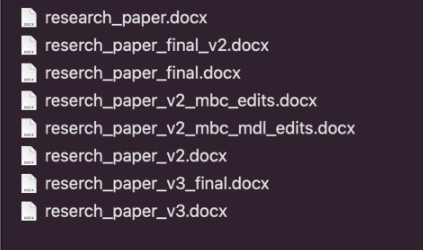
\includegraphics[width=1.41in,height=\textheight]{chapters/style_guide/../../graphics/bad_folder.png}
\end{center}

Saving a bunch of different versions of a file like this is a real mess,
and it tends to get worse the more collaborators we have. What is
contained in each document again? What order were the documents created
in? What are the differences between the documents? Does the version of
the paper that Doug emailed this morning contain the edits that Jason
made yesterday? Versioning helps us get around these problems, and
luckily, we have some good tools for versioning. Therefore, we should
generally not be emailing files to each other. Instead, we should strive
to work on Microsoft Office Documents online and use Git and GitHub for
collaborative computer programming. There are links to instructions for
both below.

\hl{Please see the Using Word SOP for instructions on how to use Word's
versioning system (Excel and PowerPoint have similar systems).}

\hl{Please see for instructions for versioning other file types with Git
and GitHub.}

\chapter{Appendix}\label{sec-appendix}

\section{Appendix A. Style Cheat
Sheet}\label{appendix-a.-style-cheat-sheet}

\begin{center}
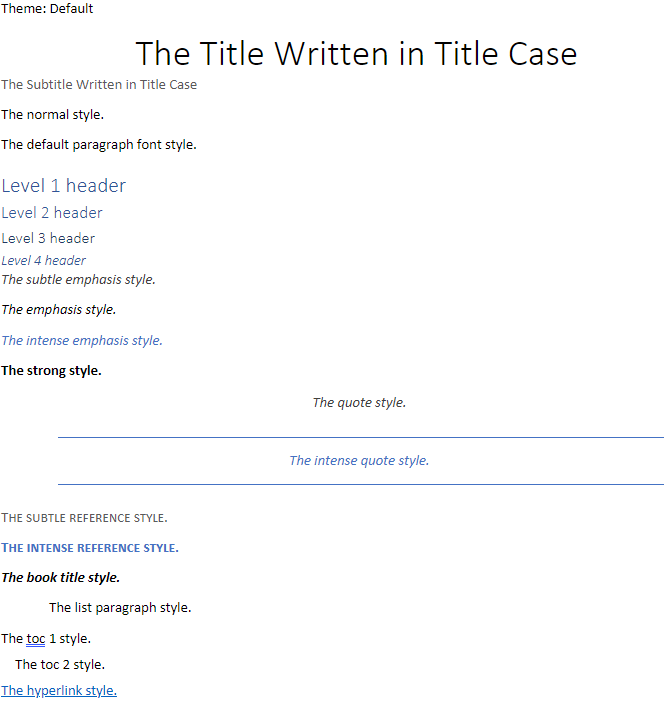
\includegraphics[width=3\textwidth,height=\textheight]{chapters/style_guide/../../graphics/style_cheat_sheet.png}
\end{center}

\section{Appendix B. UTHealth Brand
Standards}\label{appendix-b.-uthealth-brand-standards}

\subsection{Logos}\label{logos}

\href{https://www.uth.edu/brand-standards/visual-identity/index.htm}{Here
is a link to the online logo library}.

\subsection{Colors}\label{colors}

\href{https://www.uth.edu/brand-standards/visual-identity/color}{Here is
a link the color standards page.}

\begin{center}
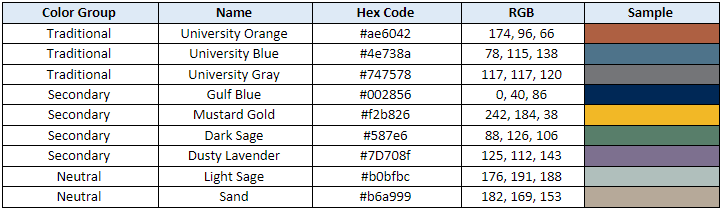
\includegraphics[width=3\textwidth,height=\textheight]{chapters/style_guide/../../graphics/ut_color_standards.png}
\end{center}

\subsection{Typefaces}\label{typefaces}

\href{https://www.uth.edu/brand-standards/visual-identity/type}{Here is
a link to the typefaces standards page}.

We don't have easy access to many of these fonts. Here are some that we
can use:

\begin{center}
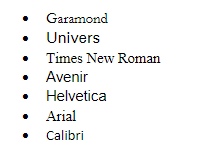
\includegraphics[width=0.3\textwidth,height=\textheight]{chapters/style_guide/../../graphics/fonts.png}
\end{center}

\bookmarksetup{startatroot}

\chapter{Getting Started with SOPs}\label{sec-sop_start}

\subsection{Overview}\label{overview}

What are SOPs and why do we need them? The following quote provides a
pretty useful answer.

\begin{quote}
\emph{A standard operating procedure (SOP) is a set of written
instructions that describes the step-by-step process that must be taken
to properly perform a routine activity. SOPs should be followed the
exact same way every time to guarantee that the organization remains
consistent and in compliance with industry regulations and business
standards.}

\emph{Standard operating procedures provide the policies, processes, and
standards needed for the organization to succeed. They can benefit a
business by reducing errors, increasing efficiencies and profitability,
creating a safe work environment, and producing guidelines for how to
resolve issues and overcome obstacles.}
\end{quote}

\emph{\href{https://www.techtarget.com/searchbusinessanalytics/definition/standard-operating-procedure-SOP}{---
Bush, 2021}}

Our team is large, diverse, and widely geographically distributed. These
traits are extremely important strengths for our team, but they also
make organizing and managing our activities more challenging than they
would be if our team were small, homogenous, and we were all located
down the hall from each other. As the quote highlights, the adoption and
use of SOPs are one way we can produce consistent, high-quality work as
often as possible. Another advantage of SOPs is that they should reduce
our cognitive load. How do SOPs reduce our cognitive load?

\begin{itemize}
\tightlist
\item
  First, they reduce the number of choices we need to make. For example,
  we don't need to come up with our own answers to questions like,
  ``where should I put this document?'' or ``what should I name this
  folder?''\\
\item
  Second, having the predetermined choices written down for reference
  reduces the amount of information we need to store in our intentional
  memory. For example, ``OK, remember to always start these file names
  with the date written as yyyy-mm-dd''. Although we don't need to
  intentionally memorize them, these predetermined choices may
  eventually bleed over into our memory by accident through
  repetition.\\
\item
  Third, having uniformly styled content makes it easier for others --
  including future us -- to find what we are looking for and use it. We
  can focus our brain power on the content instead of the style and/or
  organization of the content.
\end{itemize}

\subsection{Feedback}\label{feedback}

At the end of the day, the point of these SOPs is to make our lives
easier and improve the quality and efficiency of our work. They can't
possibly achieve any of those objectives that if they aren't used.
Therefore, we want to encourage every member of the team to provide us
with feedback. What is working? What isn't working? What's confusing?
Possibly even some positive feedback about tools and processes that
\emph{are working} -- We won't hold our breath on that one 😂. The
easiest way to send feedback is probably to just call
\href{tel:9725462925}{972-546-2925} or email
\href{mailto:Michael.B.Cannell@uth.tmc.edu}{Brad Cannell}, who is
currently responsible for maintaining the SharePoint site.

\subsection{Next Steps}\label{next-steps}

At this point, you should know what SOPs are and why we are using them.
Now what? Well, depending on your role on the team, you may rarely (if
ever) use some of the SOPs. However, any time you engage in an activity
that impacts our team or interact with a file that is shared on the
SharePoint site, there is a good chance that there is an SOP -- or soon
will be an SOP -- that provides guidelines for that activity or
interaction.

Even if you are a team member that rarely engages in an activity that is
covered in an SOP, quickly skimming through some of them may provide you
with useful information about the organization of the project that makes
your life easier.\\
Finally, these SOPs are intended to be living documents that evolve to
meet our changing needs over time. Therefore, it probably isn't a good
idea to assume that you never need to check an SOP that you've read in
the past.

Thank you for your time and consideration!

\part{Authoring SOPs}

\chapter{Overview}\label{sec-as_overview}

This part contains information about authoring SOPs. Any information we
want to record about creating, editing, or deleting SOPs should be
included in this part. Any information we want to record that is not
exclusively about creating, editing, or deleting SOPs should not be
included in this part. For example, even though SOPs use Microsoft Word,
an SOP about using Microsoft Word should be its own separate part of the
guide.

\begin{tcolorbox}[enhanced jigsaw, leftrule=.75mm, bottomrule=.15mm, toprule=.15mm, coltitle=black, title=\textcolor{quarto-callout-note-color}{\faInfo}\hspace{0.5em}{Note}, left=2mm, colback=white, opacityback=0, colbacktitle=quarto-callout-note-color!10!white, rightrule=.15mm, toptitle=1mm, breakable, bottomtitle=1mm, titlerule=0mm, arc=.35mm, opacitybacktitle=0.6, colframe=quarto-callout-note-color-frame]

We hope that all of our team members will use and provide feedback on
our SOPs; however, most of our team members will never need to author
SOPs. Most of you can safely ignore this part of the guide.

\end{tcolorbox}

Specifically, this document covers:

\begin{itemize}
\tightlist
\item
  When and how should we author SOPs?

  \begin{itemize}
  \tightlist
  \item
    Please use the
    \href{https://uthtmc.sharepoint.com/:w:/r/sites/SPHCannellResearch/Shared\%20Documents/SOPs/SOP\%20Template.docx?d=wdca3cccdecd5484cabeb5054608e5b33&csf=1&web=1&e=HiuhkD}{New
    SOP Template} to create a new SOP document.
  \item
    Please see \textbf{?@sec-sg\_overview} for general Word document
    formatting guidance.
  \end{itemize}
\item
  What technologies (apps) should we use to write our SOPs?

  \begin{itemize}
  \tightlist
  \item
    Quick Summary: SOPs should be written using Microsoft Word
    documents.
  \end{itemize}
\item
  Where should our SOPs be stored?

  \begin{itemize}
  \tightlist
  \item
    Quick Summary: SOPs should generally be stored in
    \texttt{Documents/SOPs}.
  \end{itemize}
\end{itemize}

\chapter*{Structure}\label{sec-as_structure}
\addcontentsline{toc}{chapter}{Structure}

\markboth{Structure}{Structure}

Each document should be about a single, definable topic, concept, or
technology. For example, the document you are reading right now is about
creating and editing other SOPs. Over time, we may find that what we
originally thought of as a single, definable topic, concept, or
technology is really composed of multiple different topics, concepts, or
technologies that we need to break out into separate SOP documents.
That's OK! The goal here is to make it easy to use the SOPs, and by
extension, to do good work.

The rest of the structure section of this SOP gives step-by-step
instructions for creating and authoring SOPs. It assumes that we are
starting with the New SOP Template document located in Documents/SOPs.
Note that this template has the margins set to narrow. We did this
because, although these are Word documents, we anticipate that they will
most often be viewed online. Using narrow margins gives them more of a
webpage look and feel.

\textbf{Step 1:} Start by adding a rectangular-shaped picture to the top
of the SOP document and center it. It makes the documents more appealing
to look at and feel more like reading a webpage. - To do add a picture,
click \texttt{Insert} \textgreater{} \texttt{Picture}. There are
multiple options including stock images that come with Microsoft Word.
Other useful websites for finding free pictures include Google Images
and \href{https://unsplash.com/}{Unsplash}.

\textbf{Step 2:} Immediately under the picture should be the document
title. It should succinctly capture the theme of the document. Please
apply the \texttt{Title} style to the title.

\textbf{Step 3:} Below the title, each page should have a table of
contents (TOC). The TOC should be automatically generated and link to
the document headers.

\textbf{Step 4:} Each page should also have an ``Overview'' section
under the TOC. The Overview section should contain a brief description
of the SOP's topic. If we aren't able to describe the topic in a
sentence or two, that may be an indication that the page doesn't have a
single, high-level topic.

\textbf{Step 5:} Use the header styles (i.e., Heading 1, Heading 2,
etc.) to break the document up into sections and subsections. Make sure
to use heading styles as opposed to just changing the color and font
manually. This is important for at least two reasons.

\begin{enumerate}
\def\labelenumi{\arabic{enumi}.}
\tightlist
\item
  Using a heading style will create a clickable link in the TOC (new
  headings require updating the TOC).\\
\item
  If we decide to make changes to a heading style, all of the headings
  will automatically be updated to match.
\end{enumerate}

\subsection*{Paragraphs}\label{paragraphs}
\addcontentsline{toc}{subsection}{Paragraphs}

New paragraphs, steps, and glossary items should not be indented. They
should be aligned with the left margin of the document.

\subsection*{Headers}\label{headers}
\addcontentsline{toc}{subsection}{Headers}

Each level one headings (i.e., \texttt{Heading\ 1}) should have a
single, high-level theme, but not high-level enough to (currently)
warrant its own SOP. Over time, we may find that what we originally
thought of as a single, high-level theme was really more appropriate to
break into multiple themes. That's ok.

Level one headings should be written in
\href{https://en.wikipedia.org/wiki/Title_case}{title case}. All other
headings should be written in
\href{https://en.wiktionary.org/wiki/sentence_case}{sentence case}.

\chapter*{Tone}\label{sec-tone}
\addcontentsline{toc}{chapter}{Tone}

\markboth{Tone}{Tone}

The goal is for these SOPs to be user-friendly. As such:

\begin{itemize}
\tightlist
\item
  Use informal, first-person language.
\item
  We will typically use the word ``we'' instead of the word ``I''. This
  project is a team effort.
\end{itemize}

\chapter*{Technologies}\label{sec-tech}
\addcontentsline{toc}{chapter}{Technologies}

\markboth{Technologies}{Technologies}

What technology (application), or technologies, should we use for
writing our SOPs? We've experimented, and will continue to experiment,
with many different applications, processes, and technologies for
organizing and managing all aspects of our projects -- including our
SOPs. Here is what we've found so far.

\subsection*{Using OneNote, Word Documents, and Teams/SharePoint
Pages}\label{using-onenote-word-documents-and-teamssharepoint-pages}
\addcontentsline{toc}{subsection}{Using OneNote, Word Documents, and
Teams/SharePoint Pages}

For now, we know that we want to try to manage as much of our project as
possible inside the Microsoft ecosystem. Because Microsoft products are
universally the best? Not necessarily. In fact, some members of our team
really dislike Microsoft products. Why, then? We want to manage as much
of our project as possible inside the Microsoft Ecosystem because (1)
UTHealth pays for it; (2) UTHealth IT security approves of it; (3) The
majority of our team members -- internal and external to UTHealth -- are
already familiar with, and have access to, Microsoft products.

However, even within the Microsoft ecosystem, there are often multiple
different applications and technologies we can choose to author and
store SOPs. So, which technology should we use? In the table and
paragraphs below, we list the pros and cons of using different Microsoft
technologies for creating, editing, and accessing SOPs.

\begin{figure}[H]

{\centering 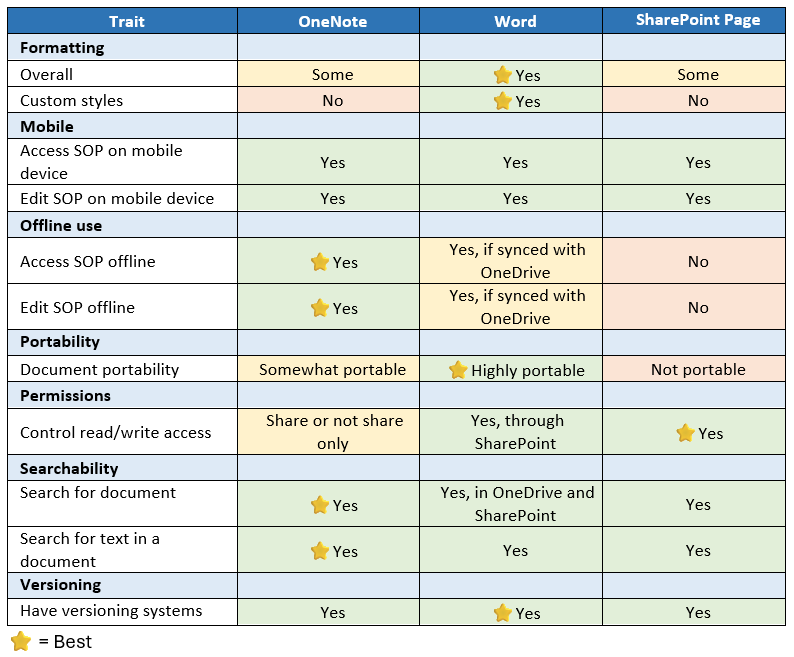
\includegraphics[width=3\textwidth,height=\textheight]{chapters/authoring_sops/../../graphics/microsoft_tech.png}

}

\caption{Summary of the pros and cons of using different Microsoft
technologies for creating, editing, and accessing SOPs. A detailed
discussion of each trait is in the sections below.}

\end{figure}%

\subsubsection*{Formatting}\label{formatting}
\addcontentsline{toc}{subsubsection}{Formatting}

When it comes to formatting the SOPS, Word has the edge over OneNote and
SharePoint pages. Word gives us finer control over formatting and more
robust tools. Especially for things like tables.

\subsubsection*{Custom Styles}\label{custom-styles}
\addcontentsline{toc}{subsubsection}{Custom Styles}

Using styles makes it so much easier to create consistently formatted
documents. OneNote, Word, and SharePoint all have some basic built-in
styles, but as of this writing, only Word allows us to create custom
styles (e.g., the \texttt{Code} style and \texttt{File\ Paths} style
available in this document). Here is a useful
\href{https://answers.microsoft.com/en-us/msoffice/forum/all/copying-style-in-word-for-the-mac/c2487cc6-901b-40a1-a445-77c598da520f}{post}
about sharing styles between Word documents.

\subsubsection*{Mobile Device Access}\label{mobile-device-access}
\addcontentsline{toc}{subsubsection}{Mobile Device Access}

Mobile device access refers to the ease with which the SOP can be
accessed and edited from a mobile device (i.e., phone or tablet).

All three technologies have a mobile app; however, the OneNote mobile
app probably provides the best overall mobile experience. It allows us
to search, read, and edit notes with the fewest number of clicks/taps.
Having said that, the difference between the three isn't large when the
app has an active internet connection.

\subsubsection*{Offline Access}\label{offline-access}
\addcontentsline{toc}{subsubsection}{Offline Access}

Offline access refers to the ease with which the SOP can be accessed and
edited in the absence of an active internet connection (e.g., when
traveling).

\paragraph*{From a desktop/laptop computer without an active internet
connection}\label{from-a-desktoplaptop-computer-without-an-active-internet-connection}
\addcontentsline{toc}{paragraph}{From a desktop/laptop computer without
an active internet connection}

OneNote provides the best experience out of the box. We can read and
edit notes in the OneNote app, which will be synced with the server when
an internet connection is reestablished. The same is true for Word
documents,
\href{https://support.microsoft.com/en-us/office/sync-sharepoint-files-with-the-onedrive-sync-client-groove-exe-59b1de2b-519e-4d3a-8f45-51647cf291cd}{but
only if they are being synced with the computer's file system}. We
highly recommend doing so. In general, SharePoint will not work without
an internet connection.

\paragraph*{From a mobile device without an active internet
connection}\label{from-a-mobile-device-without-an-active-internet-connection}
\addcontentsline{toc}{paragraph}{From a mobile device without an active
internet connection}

OneNote provides the best experience out of the box here too. We can
read and edit notes in the OneNote app, which will be synced with the
server when an internet connection is reestablished. The same is true
for Word documents,
\href{https://support.microsoft.com/en-us/office/sync-sharepoint-files-with-the-onedrive-sync-client-groove-exe-59b1de2b-519e-4d3a-8f45-51647cf291cd}{but
only if they are being synced with the computer's file system}. We
highly recommend doing so. In general, the SharePoint mobile app will
not work without an internet connection.

\subsubsection*{Portability}\label{portability}
\addcontentsline{toc}{subsubsection}{Portability}

In this context, ``portability'' refers to the ease with which the SOP
can be shared, viewed, copied, and used outside of its current context.
For example, if UTHealth decides to stop paying for Microsoft 365
tomorrow, could we access and use the SOPs?

Word documents are highly portable. OneNote is slightly less so. Why
does this matter? We never know what the technology situation will be
like tomorrow. There are a number of reasons why we could potentially
need to change the technologies and processes we are using. Therefore,
the ease with which we could migrate our content to a different
technology or process if we needed to is probably worth taking into
consideration. Additionally, we often need to collaborate with team
members outside of UTHealth. The ease with which team members who do not
have internal access to UTHealth's systems is another important
dimension or portability.

\paragraph*{\texorpdfstring{\href{https://support.microsoft.com/en-us/office/export-and-import-onenote-notebooks-a4b60da5-8f33-464e-b1ba-b95ce540f309}{Exporting
OneNote notes}}{Exporting OneNote notes}}\label{exporting-onenote-notes}
\addcontentsline{toc}{paragraph}{\href{https://support.microsoft.com/en-us/office/export-and-import-onenote-notebooks-a4b60da5-8f33-464e-b1ba-b95ce540f309}{Exporting
OneNote notes}}

\begin{itemize}
\tightlist
\item
  Exporting and importing notebooks through OneNote for the web is only
  available for notebooks stored on personal OneDrive accounts, not for
  notebooks stored on OneDrive for Business or SharePoint. For
  information about exporting notebooks to PDF files from OneNote 2016
  for Windows, see
  \href{https://support.microsoft.com/en-us/office/export-notes-from-onenote-as-a-pdf-13d173b5-7f4c-45a8-94eb-9354d63af5cd}{Export
  notes from OneNote as a PDF}.
\item
  This is kind of a big deal. If we ever need to adopt a new technology,
  migrating all of our notes out of OneNote could be very difficult.
\end{itemize}

\paragraph*{\texorpdfstring{\href{https://learn.microsoft.com/en-us/sharepoint/administration/export-a-site-list-or-document-library}{Exporting
SharePoint
pages}}{Exporting SharePoint pages}}\label{exporting-sharepoint-pages}
\addcontentsline{toc}{paragraph}{\href{https://learn.microsoft.com/en-us/sharepoint/administration/export-a-site-list-or-document-library}{Exporting
SharePoint pages}}

\begin{itemize}
\tightlist
\item
  Exporting SharePoint pages is also relatively difficult process and
  requires administrator access.
\end{itemize}

\subsubsection*{Permissions}\label{permissions}
\addcontentsline{toc}{subsubsection}{Permissions}

While we definitely value every team member's input into our SOPs,
restricting editing permissions to one or two people can be a useful
tool for maintaining the integrity of our SOPs. SharePoint has the most
robust tools for assigning user permissions. However, these user
permissions can be applied to Word documents when they are stored in a
SharePoint library.

\subsubsection*{Searching Documents}\label{searching-documents}
\addcontentsline{toc}{subsubsection}{Searching Documents}

Given the number of documents our research projects contain, the ability
to search for documents and search for text within documents is an
important consideration. We experimented with searching for documents,
and text within documents, in OneNote, Teams, and SharePoint. Here is
what we found.

\paragraph*{Searching in OneNote}\label{searching-in-onenote}
\addcontentsline{toc}{paragraph}{Searching in OneNote}

OneNote has very robust search capabilities. The screenshot below is
from the OneNote desktop app. We arbitrarily searched for the word
``during.'' OneNote returns a list of linked search results, across
notebooks, with the search team highlighted in the text.

\begin{center}
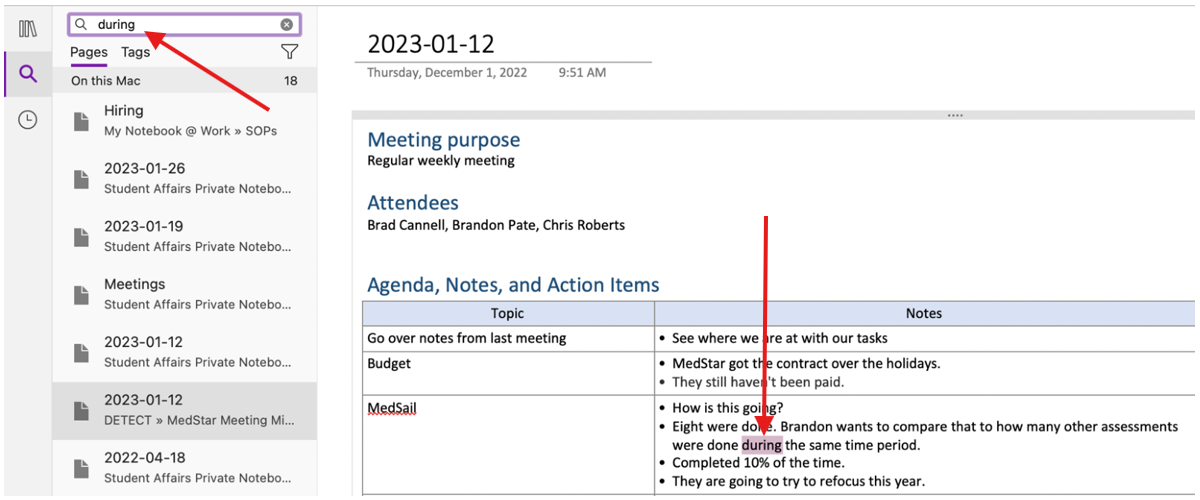
\includegraphics[width=4in,height=\textheight]{chapters/authoring_sops/../../graphics/one_note.png}
\end{center}

\paragraph*{Searching on OneDrive for
documents}\label{searching-on-onedrive-for-documents}
\addcontentsline{toc}{paragraph}{Searching on OneDrive for documents}

For this test, there was a document in OneDrive titled
🔴\hl{\href{https://uthtmc-my.sharepoint.com/:w:/r/personal/michael_b_cannell_uth_tmc_edu/Documents/02\%20Research/04\%20DETECT/DETECT\%20NIA\%20R01/03\%20Repositories/detect_clean_mdac_call_logs/issues/2023-01-20\%20Multiple\%20complete\%20Records\%20Per\%20MedStar\%20ID.docx?d=w3e7bc77253eb4f8c8c466eadd8294c59&csf=1&web=1&e=THIPrF}{2023-01-20
Multiple complete Records Per MedStar ID.docx}}. The document really
isn't that important for this example -- we just picked something. It
contains the following text, ``ID 69967''. When we navigate to
\href{https://uthtmc-my.sharepoint.com/personal/michael_b_cannell_uth_tmc_edu/_layouts/15/onedrive.aspx?login_hint=Michael\%2EB\%2ECannell\%40uth\%2Etmc\%2Eedu}{OneDrive}
and search for that text string in the search bar, the correct document
comes up in the search results. However, the exact spot where the text
appears is not shown in the search results.

\begin{center}
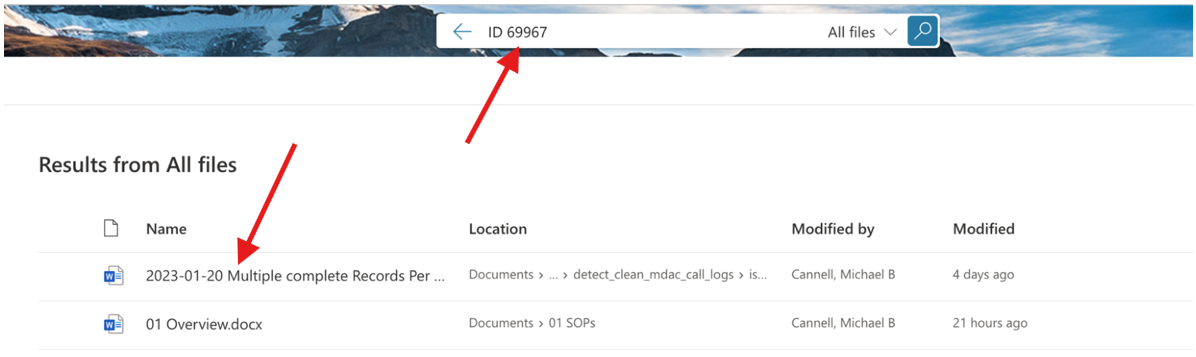
\includegraphics[width=3.99in,height=\textheight]{chapters/authoring_sops/../../graphics/one_drive.png}
\end{center}

Having said that, it isn't too big of a deal to just open the document
and do a search for the text string in the document.

\paragraph*{Searching on SharePoint for
documents}\label{searching-on-sharepoint-for-documents}
\addcontentsline{toc}{paragraph}{Searching on SharePoint for documents}

For this test, there was a document in the
\href{https://uthtmc.sharepoint.com/sites/SPHDETECT-RPC/Shared\%20Documents/Forms/AllItems.aspx?csf=1&web=1&e=FZ7xxt&FolderCTID=0x0120004E8A92AA55795C42852C8A438D043D68&viewid=37263261\%2D85dd\%2D48f3\%2D9aae\%2D93321747db5e}{DETECT
SharePoint document library} titled, 🔴\hl{SOPs.docx.} Again, there is
nothing special about this document. We're just using it as an example.
It contains the following text, ``A standard operation procedure''. When
we navigate to the
\href{https://uthtmc.sharepoint.com/sites/SPHDETECT-RPC/Shared\%20Documents/Forms/AllItems.aspx?csf=1&web=1&e=FZ7xxt&FolderCTID=0x0120004E8A92AA55795C42852C8A438D043D68&viewid=37263261\%2D85dd\%2D48f3\%2D9aae\%2D93321747db5e}{DETECT
SharePoint document library} and search for that text string in the
search bar, the correct document comes up in the search results.
However, the exact spot where the text appears is not shown in the
search results at first.

\begin{center}
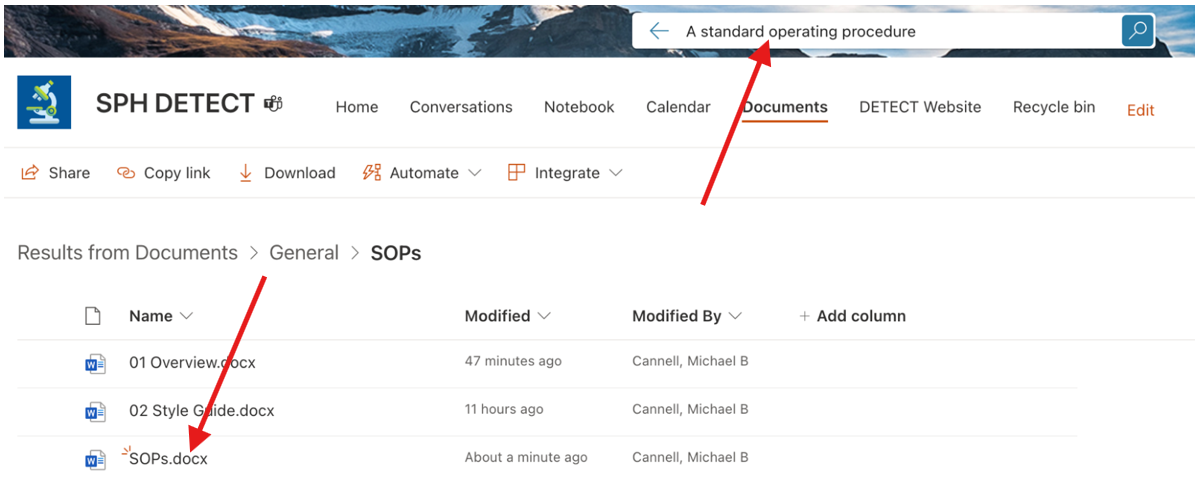
\includegraphics[width=3.99in,height=\textheight]{chapters/authoring_sops/../../graphics/share_point.png}
\end{center}

Having said that, it isn't too big of a deal to just open the document
and do a search for the text string in the document. Additionally, if we
click ``Expand search to all items in this site'' at the bottom of the
search results screen:

\begin{center}

\includegraphics[width=3.96in,height=\textheight]{chapters/authoring_sops/../../graphics/expand_search.png}
\end{center}

Then SharePoint will return a more detailed list of linked search
results that include a preview of the text string located in the
document.Graphical user interface, text, application, email

\begin{center}
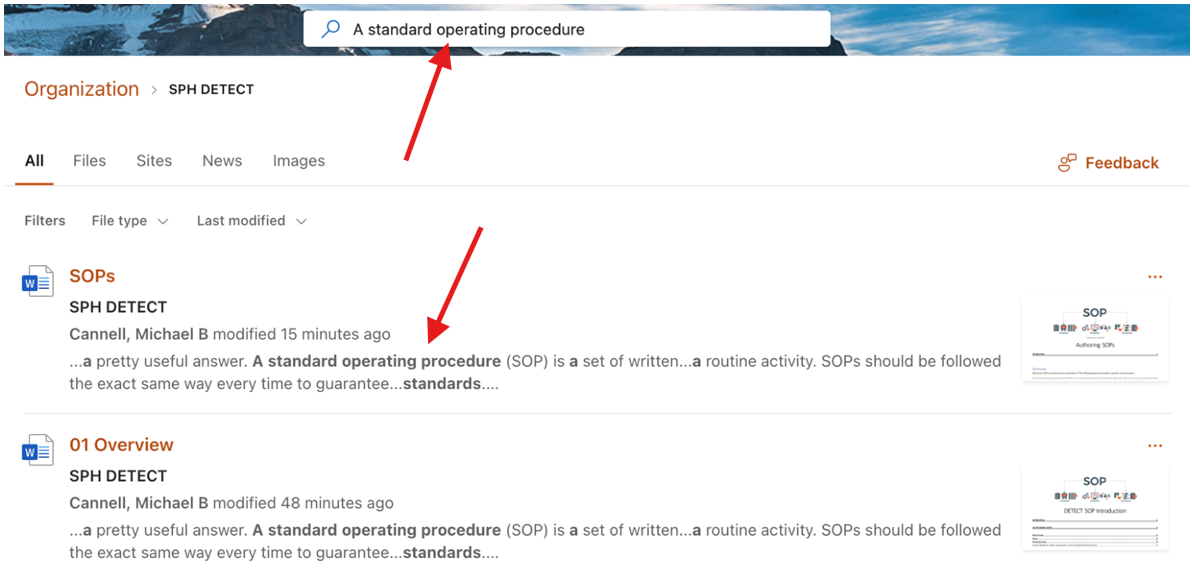
\includegraphics[width=3.97in,height=\textheight]{chapters/authoring_sops/../../graphics/sharepoint_detailed_list.png}
\end{center}

\paragraph*{Searching SharePoint
pages}\label{searching-sharepoint-pages}
\addcontentsline{toc}{paragraph}{Searching SharePoint pages}

For this test, we added a text web part to the
\href{https://uthtmc.sharepoint.com/sites/SPHDETECT-RPC/SitePages/Home.aspx}{DETECT
SharePoint homepage} that said, ``Welcome to our DETECT SharePoint
site!'' When we navigate to the DETECT SharePoint homepage and search
for that text string in the search bar, the correct document comes up in
the search results and it includes a preview of the text string located
in the document.

\begin{center}
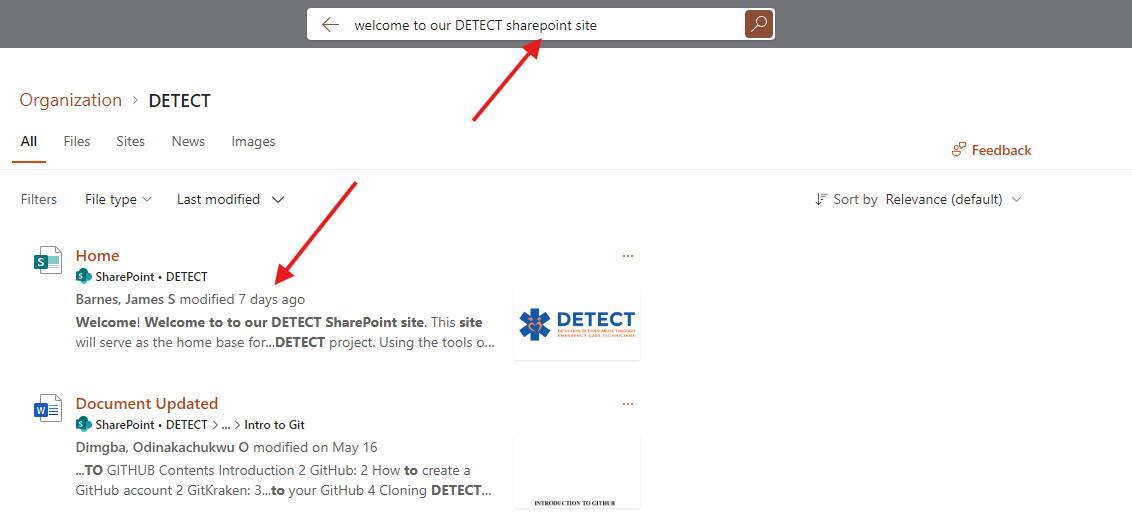
\includegraphics[width=3.77in,height=\textheight]{chapters/authoring_sops/../../graphics/sharepoint_pages.png}
\end{center}

\chapter*{Versioning}\label{sec-versioning}
\addcontentsline{toc}{chapter}{Versioning}

\markboth{Versioning}{Versioning}

Versioning is a great tool that OneNote, Word, and SharePoint pages all
have. However, Word's implementation of versioning is probably the
easiest to work with.

\subsection*{OneNote Online Versioning}\label{onenote-online-versioning}
\addcontentsline{toc}{subsection}{OneNote Online Versioning}

To see previous versions of OneNote notes, click on the \texttt{View}
tab in the ribbon and then click the \texttt{Page\ Versions} button.

\begin{center}
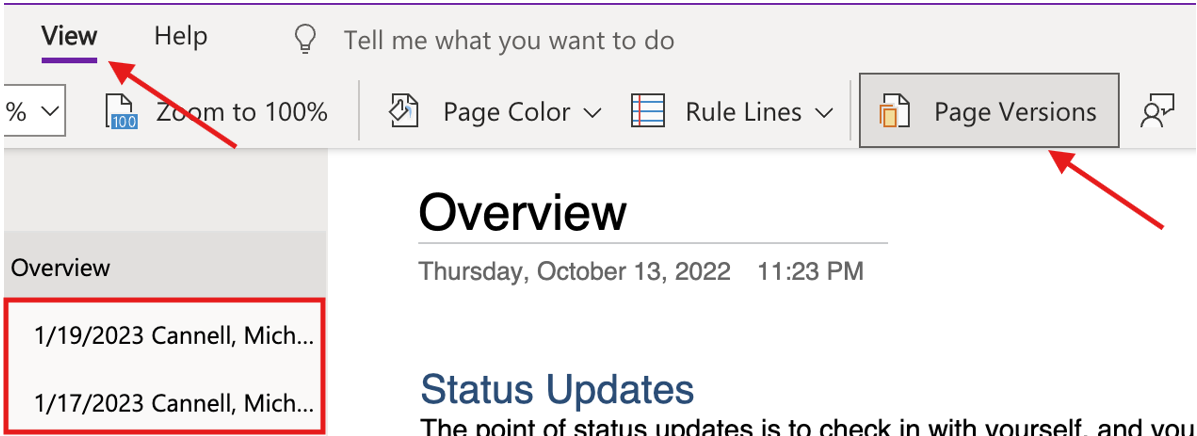
\includegraphics[width=3.99in,height=\textheight]{chapters/authoring_sops/../../graphics/onenote_versioning.png}
\end{center}

\subsection*{Word Online Versioning}\label{word-online-versioning}
\addcontentsline{toc}{subsection}{Word Online Versioning}

To use versioning in Word online, click on the document title above the
ribbon. Then, click \texttt{Version\ History}.

\begin{center}
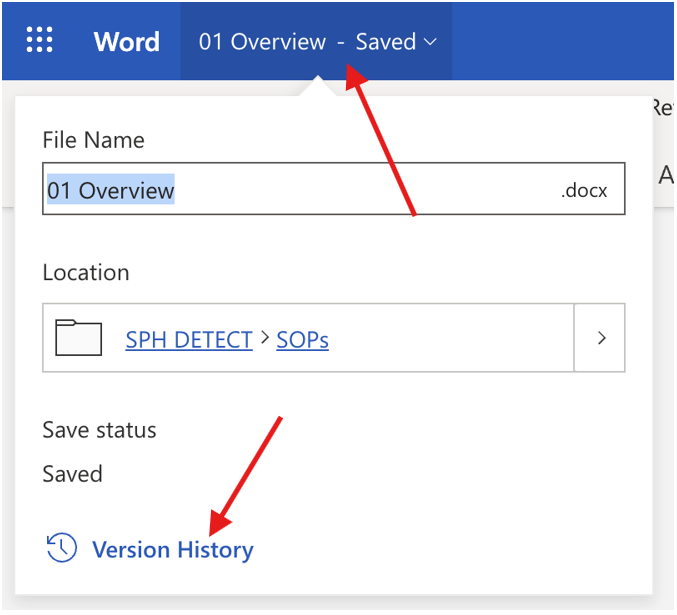
\includegraphics[width=2.26in,height=\textheight]{chapters/authoring_sops/../../graphics/word_versioning.png}
\end{center}

\subsection*{Word for Mac Versioning}\label{word-for-mac-versioning}
\addcontentsline{toc}{subsection}{Word for Mac Versioning}

To use versioning in Word for Mac, click \texttt{File} \textgreater{}
\texttt{Browse\ Version\ History}.

\begin{center}
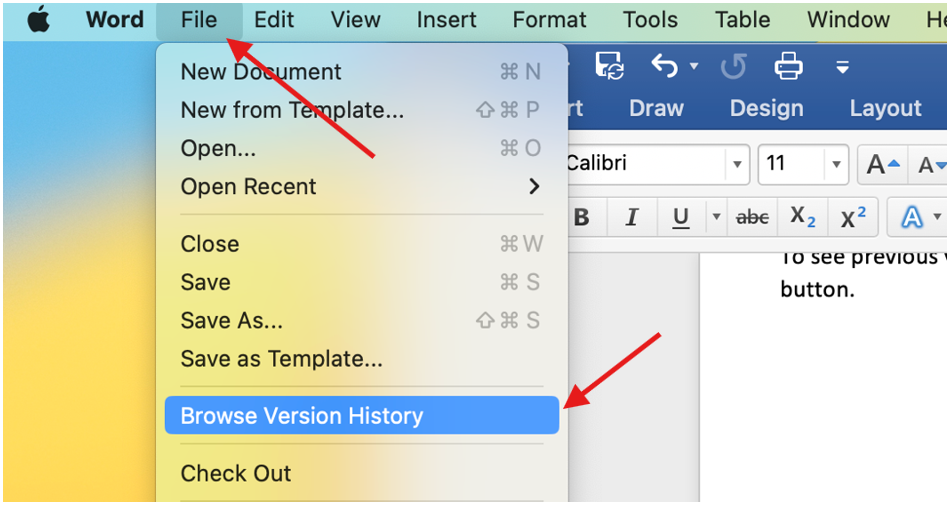
\includegraphics[width=3.17in,height=\textheight]{chapters/authoring_sops/../../graphics/word_mac_versioning.png}
\end{center}

\subsection*{SharePoint Versioning}\label{sharepoint-versioning}
\addcontentsline{toc}{subsection}{SharePoint Versioning}

To see previous versions of SharePoint pages, click \texttt{Settings}
\textgreater{} \texttt{Site\ contents} \textgreater{}
\texttt{Site\ Pages}.

\begin{center}
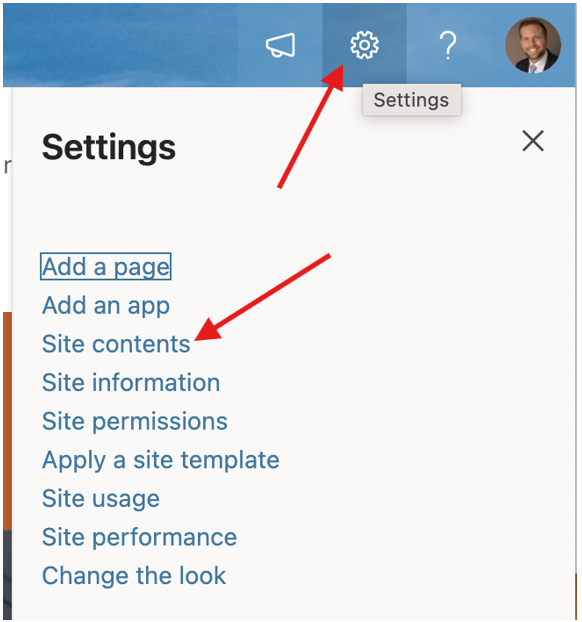
\includegraphics[width=1.94in,height=\textheight]{chapters/authoring_sops/../../graphics/sharepoint_versioning.png}
\end{center}

Find the page you want to see versions of. Then, click
\texttt{Show\ more\ actions\ for\ this\ item} (three vertically stacked
dots). Finally, click \texttt{Version\ history}.

\begin{center}
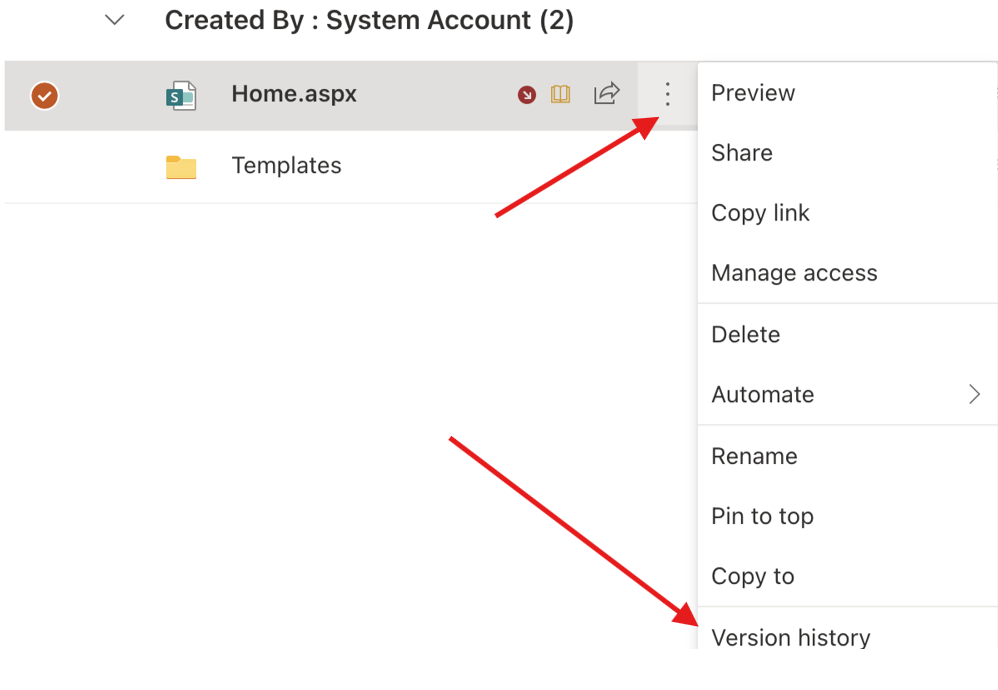
\includegraphics[width=3.33in,height=\textheight]{chapters/authoring_sops/../../graphics/sharepoint_versioning_2.png}
\end{center}



\end{document}
